\documentclass{article}
% ICML 2026 style (preprint option). Every number is a \nm{key} macro from numbers.tex, written by
% scripts/build_numbers.py from committed files; \nmst{key} gives its status. Build instructions: paper/README.md.
\usepackage{microtype}
\usepackage{graphicx}
\usepackage{booktabs}
\usepackage{xcolor}
\usepackage{hyperref}
\newcommand{\theHalgorithm}{\arabic{algorithm}}
\usepackage[preprint]{icml2026}
\usepackage{amsmath,amsfonts,amssymb}
\usepackage{url}
% Generated by scripts/build_numbers.py; do not edit. \nm{key} prints a number, \nmst{key} its status.
\makeatletter
\expandafter\def\csname nm@a5.other.benchmarks\endcsname{9}
\expandafter\def\csname nmst@a5.other.benchmarks\endcsname{record}
\expandafter\def\csname nm@a5.other.modelwins\endcsname{7}
\expandafter\def\csname nmst@a5.other.modelwins\endcsname{post hoc}
\expandafter\def\csname nm@a5.swe.indep.hi\endcsname{20}
\expandafter\def\csname nmst@a5.swe.indep.hi\endcsname{post hoc}
\expandafter\def\csname nm@a5.swe.indep.lo\endcsname{11}
\expandafter\def\csname nmst@a5.swe.indep.lo\endcsname{post hoc}
\expandafter\def\csname nm@a5.swe.model.hi\endcsname{1.8}
\expandafter\def\csname nmst@a5.swe.model.hi\endcsname{post hoc}
\expandafter\def\csname nm@a5.swe.model.lo\endcsname{1.5}
\expandafter\def\csname nmst@a5.swe.model.lo\endcsname{post hoc}
\expandafter\def\csname nm@a6.pairs\endcsname{10}
\expandafter\def\csname nmst@a6.pairs\endcsname{record}
\expandafter\def\csname nm@ah1.gap\endcsname{11.1}
\expandafter\def\csname nmst@ah1.gap\endcsname{exploratory}
\expandafter\def\csname nm@ah1.hi\endcsname{0.26}
\expandafter\def\csname nmst@ah1.hi\endcsname{exploratory}
\expandafter\def\csname nm@ah1.lo\endcsname{-0.32}
\expandafter\def\csname nmst@ah1.lo\endcsname{exploratory}
\expandafter\def\csname nm@ah1.r\endcsname{0.02}
\expandafter\def\csname nmst@ah1.r\endcsname{exploratory}
\expandafter\def\csname nm@ah2.haiku.diff\endcsname{3.7}
\expandafter\def\csname nmst@ah2.haiku.diff\endcsname{confirmatory}
\expandafter\def\csname nm@ah2.haiku.hi\endcsname{6.2}
\expandafter\def\csname nmst@ah2.haiku.hi\endcsname{confirmatory}
\expandafter\def\csname nm@ah2.haiku.k\endcsname{2}
\expandafter\def\csname nmst@ah2.haiku.k\endcsname{confirmatory}
\expandafter\def\csname nm@ah2.haiku.lo\endcsname{1.3}
\expandafter\def\csname nmst@ah2.haiku.lo\endcsname{confirmatory}
\expandafter\def\csname nm@ah2.haiku.ratio\endcsname{1.17}
\expandafter\def\csname nmst@ah2.haiku.ratio\endcsname{confirmatory}
\expandafter\def\csname nm@ah2.haiku.vs3\endcsname{1.8}
\expandafter\def\csname nmst@ah2.haiku.vs3\endcsname{exploratory}
\expandafter\def\csname nm@ah2.haiku.vs3hi\endcsname{4.3}
\expandafter\def\csname nmst@ah2.haiku.vs3hi\endcsname{exploratory}
\expandafter\def\csname nm@ah2.haiku.vs3lo\endcsname{-0.7}
\expandafter\def\csname nmst@ah2.haiku.vs3lo\endcsname{exploratory}
\expandafter\def\csname nm@ah2.luna.diff\endcsname{10.7}
\expandafter\def\csname nmst@ah2.luna.diff\endcsname{confirmatory}
\expandafter\def\csname nm@ah2.luna.hi\endcsname{14.2}
\expandafter\def\csname nmst@ah2.luna.hi\endcsname{confirmatory}
\expandafter\def\csname nm@ah2.luna.k\endcsname{3}
\expandafter\def\csname nmst@ah2.luna.k\endcsname{confirmatory}
\expandafter\def\csname nm@ah2.luna.lo\endcsname{7.1}
\expandafter\def\csname nmst@ah2.luna.lo\endcsname{confirmatory}
\expandafter\def\csname nm@ah2.luna.ratio\endcsname{1.38}
\expandafter\def\csname nmst@ah2.luna.ratio\endcsname{confirmatory}
\expandafter\def\csname nm@ah2.luna.vs3\endcsname{10.7}
\expandafter\def\csname nmst@ah2.luna.vs3\endcsname{exploratory}
\expandafter\def\csname nm@ah2.luna.vs3hi\endcsname{14.2}
\expandafter\def\csname nmst@ah2.luna.vs3hi\endcsname{exploratory}
\expandafter\def\csname nm@ah2.luna.vs3lo\endcsname{7.1}
\expandafter\def\csname nmst@ah2.luna.vs3lo\endcsname{exploratory}
\expandafter\def\csname nm@ah2.p\endcsname{0.001}
\expandafter\def\csname nmst@ah2.p\endcsname{confirmatory}
\expandafter\def\csname nm@ah2.p.holm\endcsname{0.001}
\expandafter\def\csname nmst@ah2.p.holm\endcsname{confirmatory}
\expandafter\def\csname nm@ah3.gain\endcsname{0.7}
\expandafter\def\csname nmst@ah3.gain\endcsname{confirmatory}
\expandafter\def\csname nm@ah3.gain.hi\endcsname{2.6}
\expandafter\def\csname nmst@ah3.gain.hi\endcsname{confirmatory}
\expandafter\def\csname nm@ah3.gain.lo\endcsname{0.4}
\expandafter\def\csname nmst@ah3.gain.lo\endcsname{confirmatory}
\expandafter\def\csname nm@ah3.gainupper\endcsname{1.3}
\expandafter\def\csname nmst@ah3.gainupper\endcsname{confirmatory}
\expandafter\def\csname nm@ah3.mae\endcsname{0.8}
\expandafter\def\csname nmst@ah3.mae\endcsname{confirmatory}
\expandafter\def\csname nm@ah3.upper\endcsname{2.4}
\expandafter\def\csname nmst@ah3.upper\endcsname{confirmatory}
\expandafter\def\csname nm@ah4.diff\endcsname{0.71}
\expandafter\def\csname nmst@ah4.diff\endcsname{exploratory}
\expandafter\def\csname nm@ah4.easy\endcsname{0.85}
\expandafter\def\csname nmst@ah4.easy\endcsname{exploratory}
\expandafter\def\csname nm@ah4.hard\endcsname{0.14}
\expandafter\def\csname nmst@ah4.hard\endcsname{exploratory}
\expandafter\def\csname nm@ah4.hi\endcsname{1.05}
\expandafter\def\csname nmst@ah4.hi\endcsname{exploratory}
\expandafter\def\csname nm@ah4.lo\endcsname{0.41}
\expandafter\def\csname nmst@ah4.lo\endcsname{exploratory}
\expandafter\def\csname nm@anchor.items.all\endcsname{533}
\expandafter\def\csname nmst@anchor.items.all\endcsname{record}
\expandafter\def\csname nm@anchor.items.bbeh\endcsname{440}
\expandafter\def\csname nmst@anchor.items.bbeh\endcsname{record}
\expandafter\def\csname nm@anchor.items.math\endcsname{93}
\expandafter\def\csname nmst@anchor.items.math\endcsname{record}
\expandafter\def\csname nm@anchor.share.all\endcsname{0.61}
\expandafter\def\csname nmst@anchor.share.all\endcsname{exploratory}
\expandafter\def\csname nm@anchor.share.bbeh\endcsname{0.65}
\expandafter\def\csname nmst@anchor.share.bbeh\endcsname{exploratory}
\expandafter\def\csname nm@anchor.share.math\endcsname{0.43}
\expandafter\def\csname nmst@anchor.share.math\endcsname{exploratory}
\expandafter\def\csname nm@anchor.sol.all\endcsname{56.2}
\expandafter\def\csname nmst@anchor.sol.all\endcsname{exploratory}
\expandafter\def\csname nm@anchor.sol.bbeh\endcsname{60.6}
\expandafter\def\csname nmst@anchor.sol.bbeh\endcsname{exploratory}
\expandafter\def\csname nm@anchor.sol.bbeh.usd\endcsname{\$0.0024}
\expandafter\def\csname nmst@anchor.sol.bbeh.usd\endcsname{exploratory}
\expandafter\def\csname nm@anchor.sol.math\endcsname{35.1}
\expandafter\def\csname nmst@anchor.sol.math\endcsname{exploratory}
\expandafter\def\csname nm@anchor.sol.math.usd\endcsname{\$0.032}
\expandafter\def\csname nmst@anchor.sol.math.usd\endcsname{exploratory}
\expandafter\def\csname nm@anchor.sol3.all\endcsname{58.7}
\expandafter\def\csname nmst@anchor.sol3.all\endcsname{exploratory}
\expandafter\def\csname nm@anchor.sol3.bbeh\endcsname{62.1}
\expandafter\def\csname nmst@anchor.sol3.bbeh\endcsname{exploratory}
\expandafter\def\csname nm@anchor.sol3.math\endcsname{43.0}
\expandafter\def\csname nmst@anchor.sol3.math\endcsname{exploratory}
\expandafter\def\csname nm@anchor.sol3.math.usd\endcsname{\$0.096}
\expandafter\def\csname nmst@anchor.sol3.math.usd\endcsname{exploratory}
\expandafter\def\csname nm@anchor.solmed.bbeh\endcsname{60.9}
\expandafter\def\csname nmst@anchor.solmed.bbeh\endcsname{exploratory}
\expandafter\def\csname nm@atlas.bbeh.items\endcsname{300}
\expandafter\def\csname nmst@atlas.bbeh.items\endcsname{record}
\expandafter\def\csname nm@atlas.bbeh.share\endcsname{0.42}
\expandafter\def\csname nmst@atlas.bbeh.share\endcsname{post hoc}
\expandafter\def\csname nm@atlas.bbeh.systems\endcsname{4}
\expandafter\def\csname nmst@atlas.bbeh.systems\endcsname{record}
\expandafter\def\csname nm@atlas.lb.items\endcsname{228}
\expandafter\def\csname nmst@atlas.lb.items\endcsname{record}
\expandafter\def\csname nm@atlas.lb.share\endcsname{0.65}
\expandafter\def\csname nmst@atlas.lb.share\endcsname{post hoc}
\expandafter\def\csname nm@atlas.lb.systems\endcsname{165}
\expandafter\def\csname nmst@atlas.lb.systems\endcsname{record}
\expandafter\def\csname nm@atlas.ma.items\endcsname{733}
\expandafter\def\csname nmst@atlas.ma.items\endcsname{record}
\expandafter\def\csname nm@atlas.ma.sets\endcsname{23}
\expandafter\def\csname nmst@atlas.ma.sets\endcsname{record}
\expandafter\def\csname nm@atlas.ma.share\endcsname{0.73}
\expandafter\def\csname nmst@atlas.ma.share\endcsname{post hoc}
\expandafter\def\csname nm@atlas.ma.systems\endcsname{126}
\expandafter\def\csname nmst@atlas.ma.systems\endcsname{record}
\expandafter\def\csname nm@atlas.public.items\endcsname{1,461}
\expandafter\def\csname nmst@atlas.public.items\endcsname{record}
\expandafter\def\csname nm@atlas.public.systems\endcsname{464}
\expandafter\def\csname nmst@atlas.public.systems\endcsname{record}
\expandafter\def\csname nm@atlas.swe.items\endcsname{500}
\expandafter\def\csname nmst@atlas.swe.items\endcsname{record}
\expandafter\def\csname nm@atlas.swe.share\endcsname{0.73}
\expandafter\def\csname nmst@atlas.swe.share\endcsname{post hoc}
\expandafter\def\csname nm@atlas.swe.systems\endcsname{173}
\expandafter\def\csname nmst@atlas.swe.systems\endcsname{record}
\expandafter\def\csname nm@audits.adjust\endcsname{74}
\expandafter\def\csname nmst@audits.adjust\endcsname{record}
\expandafter\def\csname nm@audits.count\endcsname{101}
\expandafter\def\csname nmst@audits.count\endcsname{record}
\expandafter\def\csname nm@audits.go\endcsname{26}
\expandafter\def\csname nmst@audits.go\endcsname{record}
\expandafter\def\csname nm@audits.stop\endcsname{1}
\expandafter\def\csname nmst@audits.stop\endcsname{record}
\expandafter\def\csname nm@cd.status\endcsname{pending}
\expandafter\def\csname nmst@cd.status\endcsname{pending}
\expandafter\def\csname nm@check.haiku.accept\endcsname{66}
\expandafter\def\csname nmst@check.haiku.accept\endcsname{exploratory}
\expandafter\def\csname nm@check.haiku.auroc\endcsname{0.78}
\expandafter\def\csname nmst@check.haiku.auroc\endcsname{exploratory}
\expandafter\def\csname nm@check.haiku.n\endcsname{523}
\expandafter\def\csname nmst@check.haiku.n\endcsname{record}
\expandafter\def\csname nm@check.sol.accept\endcsname{97}
\expandafter\def\csname nmst@check.sol.accept\endcsname{exploratory}
\expandafter\def\csname nm@check.sol.auroc\endcsname{0.69}
\expandafter\def\csname nmst@check.sol.auroc\endcsname{exploratory}
\expandafter\def\csname nm@check.sol.n\endcsname{500}
\expandafter\def\csname nmst@check.sol.n\endcsname{record}
\expandafter\def\csname nm@cited.cofailure.under\endcsname{2.5}
\expandafter\def\csname nmst@cited.cofailure.under\endcsname{cited}
\expandafter\def\csname nm@design.boot\endcsname{200}
\expandafter\def\csname nmst@design.boot\endcsname{design}
\expandafter\def\csname nm@design.gainpoints\endcsname{3}
\expandafter\def\csname nmst@design.gainpoints\endcsname{design}
\expandafter\def\csname nm@design.halves\endcsname{40}
\expandafter\def\csname nmst@design.halves\endcsname{design}
\expandafter\def\csname nm@design.near\endcsname{1.5}
\expandafter\def\csname nmst@design.near\endcsname{design}
\expandafter\def\csname nm@design.p4.items\endcsname{150}
\expandafter\def\csname nmst@design.p4.items\endcsname{design}
\expandafter\def\csname nm@design.p4.others0\endcsname{0.3}
\expandafter\def\csname nmst@design.p4.others0\endcsname{design}
\expandafter\def\csname nm@design.p4.others1\endcsname{0.5}
\expandafter\def\csname nmst@design.p4.others1\endcsname{design}
\expandafter\def\csname nm@design.p4.others2\endcsname{0.7}
\expandafter\def\csname nmst@design.p4.others2\endcsname{design}
\expandafter\def\csname nm@design.p4.reps\endcsname{8}
\expandafter\def\csname nmst@design.p4.reps\endcsname{design}
\expandafter\def\csname nm@design.p4.share0\endcsname{0.07}
\expandafter\def\csname nmst@design.p4.share0\endcsname{design}
\expandafter\def\csname nm@design.p4.share1\endcsname{0.55}
\expandafter\def\csname nmst@design.p4.share1\endcsname{design}
\expandafter\def\csname nm@design.p4.systems0\endcsname{3}
\expandafter\def\csname nmst@design.p4.systems0\endcsname{design}
\expandafter\def\csname nm@design.p4.systems1\endcsname{5}
\expandafter\def\csname nmst@design.p4.systems1\endcsname{design}
\expandafter\def\csname nm@design.p4.systems2\endcsname{9}
\expandafter\def\csname nmst@design.p4.systems2\endcsname{design}
\expandafter\def\csname nm@design.p4.top\endcsname{0.85}
\expandafter\def\csname nmst@design.p4.top\endcsname{design}
\expandafter\def\csname nm@design.p8.ma.items.hi\endcsname{26}
\expandafter\def\csname nmst@design.p8.ma.items.hi\endcsname{record}
\expandafter\def\csname nm@design.p8.ma.items.lo\endcsname{15}
\expandafter\def\csname nmst@design.p8.ma.items.lo\endcsname{record}
\expandafter\def\csname nm@design.power.min\endcsname{0.70}
\expandafter\def\csname nmst@design.power.min\endcsname{design}
\expandafter\def\csname nm@design.ridge\endcsname{0.1}
\expandafter\def\csname nmst@design.ridge\endcsname{design}
\expandafter\def\csname nm@design.sets.hi\endcsname{5}
\expandafter\def\csname nmst@design.sets.hi\endcsname{design}
\expandafter\def\csname nm@design.sets.lo\endcsname{2}
\expandafter\def\csname nmst@design.sets.lo\endcsname{design}
\expandafter\def\csname nm@design.weak.hi\endcsname{0.7}
\expandafter\def\csname nmst@design.weak.hi\endcsname{design}
\expandafter\def\csname nm@design.weak.lo\endcsname{0.2}
\expandafter\def\csname nmst@design.weak.lo\endcsname{design}
\expandafter\def\csname nm@f1.calls\endcsname{5}
\expandafter\def\csname nmst@f1.calls\endcsname{record}
\expandafter\def\csname nm@f1.neff5\endcsname{1.84}
\expandafter\def\csname nmst@f1.neff5\endcsname{preregistered-descriptive}
\expandafter\def\csname nm@f1.rho\endcsname{0.43}
\expandafter\def\csname nmst@f1.rho\endcsname{preregistered-descriptive}
\expandafter\def\csname nm@f10.off\endcsname{40}
\expandafter\def\csname nmst@f10.off\endcsname{exploratory}
\expandafter\def\csname nm@f10.on\endcsname{75}
\expandafter\def\csname nmst@f10.on\endcsname{exploratory}
\expandafter\def\csname nm@f11.sol.est\endcsname{62.5}
\expandafter\def\csname nmst@f11.sol.est\endcsname{exploratory}
\expandafter\def\csname nm@f11.sol.true\endcsname{97.3}
\expandafter\def\csname nmst@f11.sol.true\endcsname{exploratory}
\expandafter\def\csname nm@f12.agg\endcsname{0.236}
\expandafter\def\csname nmst@f12.agg\endcsname{exploratory}
\expandafter\def\csname nm@f12.vote\endcsname{0.189}
\expandafter\def\csname nmst@f12.vote\endcsname{exploratory}
\expandafter\def\csname nm@f16.fake\endcsname{5.2}
\expandafter\def\csname nmst@f16.fake\endcsname{record}
\expandafter\def\csname nm@f17.allwrong.copula\endcsname{5.5}
\expandafter\def\csname nmst@f17.allwrong.copula\endcsname{post hoc}
\expandafter\def\csname nm@f17.allwrong.indep\endcsname{0.0}
\expandafter\def\csname nmst@f17.allwrong.indep\endcsname{post hoc}
\expandafter\def\csname nm@f17.allwrong.l0\endcsname{6.1}
\expandafter\def\csname nmst@f17.allwrong.l0\endcsname{post hoc}
\expandafter\def\csname nm@f17.allwrong.l1\endcsname{8.5}
\expandafter\def\csname nmst@f17.allwrong.l1\endcsname{post hoc}
\expandafter\def\csname nm@f17.allwrong.obs\endcsname{8.6}
\expandafter\def\csname nmst@f17.allwrong.obs\endcsname{post hoc}
\expandafter\def\csname nm@f17.corr.l0\endcsname{0.502}
\expandafter\def\csname nmst@f17.corr.l0\endcsname{post hoc}
\expandafter\def\csname nm@f17.corr.obs\endcsname{0.512}
\expandafter\def\csname nmst@f17.corr.obs\endcsname{post hoc}
\expandafter\def\csname nm@f17.difficulty.share\endcsname{98}
\expandafter\def\csname nmst@f17.difficulty.share\endcsname{post hoc}
\expandafter\def\csname nm@f17.samecompany\endcsname{0.026}
\expandafter\def\csname nmst@f17.samecompany\endcsname{post hoc}
\expandafter\def\csname nm@f17.share\endcsname{0.69}
\expandafter\def\csname nmst@f17.share\endcsname{post hoc}
\expandafter\def\csname nm@f17.systems\endcsname{39}
\expandafter\def\csname nmst@f17.systems\endcsname{record}
\expandafter\def\csname nm@f18.best\endcsname{76.8}
\expandafter\def\csname nmst@f18.best\endcsname{post hoc}
\expandafter\def\csname nm@f18.cover2\endcsname{84.0}
\expandafter\def\csname nmst@f18.cover2\endcsname{post hoc}
\expandafter\def\csname nm@f18.cover39\endcsname{91.4}
\expandafter\def\csname nmst@f18.cover39\endcsname{post hoc}
\expandafter\def\csname nm@f18.minimax.acc\endcsname{75.8}
\expandafter\def\csname nmst@f18.minimax.acc\endcsname{post hoc}
\expandafter\def\csname nm@f18.minimax.usd\endcsname{\$0.073}
\expandafter\def\csname nmst@f18.minimax.usd\endcsname{post hoc}
\expandafter\def\csname nm@f18.opus.acc\endcsname{76.8}
\expandafter\def\csname nmst@f18.opus.acc\endcsname{post hoc}
\expandafter\def\csname nm@f18.opus.usd\endcsname{\$0.754}
\expandafter\def\csname nmst@f18.opus.usd\endcsname{post hoc}
\expandafter\def\csname nm@f18.price.ratio\endcsname{10}
\expandafter\def\csname nmst@f18.price.ratio\endcsname{post hoc}
\expandafter\def\csname nm@f18.stepauroc\endcsname{0.68}
\expandafter\def\csname nmst@f18.stepauroc\endcsname{post hoc}
\expandafter\def\csname nm@f2.neff12\endcsname{3.74}
\expandafter\def\csname nmst@f2.neff12\endcsname{preregistered-descriptive}
\expandafter\def\csname nm@f3.haiku.acc\endcsname{43.3}
\expandafter\def\csname nmst@f3.haiku.acc\endcsname{preregistered-descriptive}
\expandafter\def\csname nm@f3.luna.acc\endcsname{19.3}
\expandafter\def\csname nmst@f3.luna.acc\endcsname{preregistered-descriptive}
\expandafter\def\csname nm@f3.sol.acc\endcsname{97.3}
\expandafter\def\csname nmst@f3.sol.acc\endcsname{preregistered-descriptive}
\expandafter\def\csname nm@f3.sol.usd\endcsname{\$0.0062}
\expandafter\def\csname nmst@f3.sol.usd\endcsname{preregistered-descriptive}
\expandafter\def\csname nm@f3.sonnet.acc\endcsname{72.0}
\expandafter\def\csname nmst@f3.sonnet.acc\endcsname{preregistered-descriptive}
\expandafter\def\csname nm@f3.sonnet.usd\endcsname{\$0.0139}
\expandafter\def\csname nmst@f3.sonnet.usd\endcsname{preregistered-descriptive}
\expandafter\def\csname nm@f4.cascades\endcsname{276}
\expandafter\def\csname nmst@f4.cascades\endcsname{post hoc}
\expandafter\def\csname nm@f4.dollars\endcsname{0.8}
\expandafter\def\csname nmst@f4.dollars\endcsname{post hoc}
\expandafter\def\csname nm@f4.haiku5\endcsname{48.3}
\expandafter\def\csname nmst@f4.haiku5\endcsname{exploratory}
\expandafter\def\csname nm@f4.panel.calls\endcsname{12}
\expandafter\def\csname nmst@f4.panel.calls\endcsname{record}
\expandafter\def\csname nm@f4.panel12\endcsname{58.0}
\expandafter\def\csname nmst@f4.panel12\endcsname{exploratory}
\expandafter\def\csname nm@f4.within\endcsname{2}
\expandafter\def\csname nmst@f4.within\endcsname{post hoc}
\expandafter\def\csname nm@f5.diff\endcsname{-0.7}
\expandafter\def\csname nmst@f5.diff\endcsname{confirmatory}
\expandafter\def\csname nm@f5.escalates\endcsname{78}
\expandafter\def\csname nmst@f5.escalates\endcsname{confirmatory}
\expandafter\def\csname nm@f7.of\endcsname{40}
\expandafter\def\csname nmst@f7.of\endcsname{preregistered-descriptive}
\expandafter\def\csname nm@f7.perturbed\endcsname{40}
\expandafter\def\csname nmst@f7.perturbed\endcsname{preregistered-descriptive}
\expandafter\def\csname nm@f9.diff\endcsname{0.0061}
\expandafter\def\csname nmst@f9.diff\endcsname{exploratory}
\expandafter\def\csname nm@judge.haiku.below\endcsname{3.3}
\expandafter\def\csname nmst@judge.haiku.below\endcsname{post hoc}
\expandafter\def\csname nm@judge.haiku.vsown\endcsname{-3.3}
\expandafter\def\csname nmst@judge.haiku.vsown\endcsname{post hoc}
\expandafter\def\csname nm@judge.sol.bbeh.acc\endcsname{52.3}
\expandafter\def\csname nmst@judge.sol.bbeh.acc\endcsname{exploratory}
\expandafter\def\csname nm@judge.sol.bbeh.bestpool\endcsname{38.9}
\expandafter\def\csname nmst@judge.sol.bbeh.bestpool\endcsname{exploratory}
\expandafter\def\csname nm@judge.sol.bbeh.coverage\endcsname{58.0}
\expandafter\def\csname nmst@judge.sol.bbeh.coverage\endcsname{exploratory}
\expandafter\def\csname nm@judge.sol.bbeh.eta\endcsname{0.70}
\expandafter\def\csname nmst@judge.sol.bbeh.eta\endcsname{exploratory}
\expandafter\def\csname nm@judge.sol.bbeh.etahi\endcsname{0.80}
\expandafter\def\csname nmst@judge.sol.bbeh.etahi\endcsname{exploratory}
\expandafter\def\csname nm@judge.sol.bbeh.etalo\endcsname{0.57}
\expandafter\def\csname nmst@judge.sol.bbeh.etalo\endcsname{exploratory}
\expandafter\def\csname nm@judge.sol.bbeh.usd\endcsname{\$0.0040}
\expandafter\def\csname nmst@judge.sol.bbeh.usd\endcsname{exploratory}
\expandafter\def\csname nm@judge.sol.bbeh.vsbest\endcsname{13.3}
\expandafter\def\csname nmst@judge.sol.bbeh.vsbest\endcsname{exploratory}
\expandafter\def\csname nm@judge.sol.bbeh.vsbesthi\endcsname{15.8}
\expandafter\def\csname nmst@judge.sol.bbeh.vsbesthi\endcsname{exploratory}
\expandafter\def\csname nm@judge.sol.bbeh.vsbestlo\endcsname{9.8}
\expandafter\def\csname nmst@judge.sol.bbeh.vsbestlo\endcsname{exploratory}
\expandafter\def\csname nm@judge.sol.bbeh.vsplur\endcsname{8.5}
\expandafter\def\csname nmst@judge.sol.bbeh.vsplur\endcsname{exploratory}
\expandafter\def\csname nm@judge.sol.below\endcsname{8.3}
\expandafter\def\csname nmst@judge.sol.below\endcsname{post hoc}
\expandafter\def\csname nm@judge.sol.math.coverage\endcsname{22.6}
\expandafter\def\csname nmst@judge.sol.math.coverage\endcsname{exploratory}
\expandafter\def\csname nm@judge.sol.math.vsbest\endcsname{2.9}
\expandafter\def\csname nmst@judge.sol.math.vsbest\endcsname{exploratory}
\expandafter\def\csname nm@judge.sol.vsown\endcsname{-8.3}
\expandafter\def\csname nmst@judge.sol.vsown\endcsname{post hoc}
\expandafter\def\csname nm@judge.sol.vsown.hi\endcsname{-4.8}
\expandafter\def\csname nmst@judge.sol.vsown.hi\endcsname{post hoc}
\expandafter\def\csname nm@judge.sol.vsown.lo\endcsname{-12.0}
\expandafter\def\csname nmst@judge.sol.vsown.lo\endcsname{post hoc}
\expandafter\def\csname nm@judge.sol.vsown.ratio\endcsname{1.6}
\expandafter\def\csname nmst@judge.sol.vsown.ratio\endcsname{post hoc}
\expandafter\def\csname nm@lf.answer\endcsname{47.5}
\expandafter\def\csname nmst@lf.answer\endcsname{exploratory}
\expandafter\def\csname nm@lf.sonnet.est\endcsname{79}
\expandafter\def\csname nmst@lf.sonnet.est\endcsname{exploratory}
\expandafter\def\csname nm@lf.sonnet.true\endcsname{45}
\expandafter\def\csname nmst@lf.sonnet.true\endcsname{exploratory}
\expandafter\def\csname nm@p1.all.cells\endcsname{695}
\expandafter\def\csname nmst@p1.all.cells\endcsname{record}
\expandafter\def\csname nm@p1.all.corr\endcsname{0.46}
\expandafter\def\csname nmst@p1.all.corr\endcsname{post hoc}
\expandafter\def\csname nm@p1.all.levmsed\endcsname{-4.2}
\expandafter\def\csname nmst@p1.all.levmsed\endcsname{post hoc}
\expandafter\def\csname nm@p1.all.levmsedhi\endcsname{-1.6}
\expandafter\def\csname nmst@p1.all.levmsedhi\endcsname{post hoc}
\expandafter\def\csname nm@p1.all.levmsedlo\endcsname{-9.1}
\expandafter\def\csname nmst@p1.all.levmsedlo\endcsname{post hoc}
\expandafter\def\csname nm@p1.all.levrule\endcsname{4.4}
\expandafter\def\csname nmst@p1.all.levrule\endcsname{post hoc}
\expandafter\def\csname nm@p1.all.levzero\endcsname{4.0}
\expandafter\def\csname nmst@p1.all.levzero\endcsname{post hoc}
\expandafter\def\csname nm@p1.all.msed\endcsname{2.4}
\expandafter\def\csname nmst@p1.all.msed\endcsname{post hoc}
\expandafter\def\csname nm@p1.all.msedhi\endcsname{3.4}
\expandafter\def\csname nmst@p1.all.msedhi\endcsname{post hoc}
\expandafter\def\csname nm@p1.all.msedlo\endcsname{0.6}
\expandafter\def\csname nmst@p1.all.msedlo\endcsname{post hoc}
\expandafter\def\csname nm@p1.all.obsgain\endcsname{1.8}
\expandafter\def\csname nmst@p1.all.obsgain\endcsname{post hoc}
\expandafter\def\csname nm@p1.all.predgain\endcsname{2.8}
\expandafter\def\csname nmst@p1.all.predgain\endcsname{post hoc}
\expandafter\def\csname nm@p1.all.rule\endcsname{2.0}
\expandafter\def\csname nmst@p1.all.rule\endcsname{post hoc}
\expandafter\def\csname nm@p1.all.sets\endcsname{24}
\expandafter\def\csname nmst@p1.all.sets\endcsname{record}
\expandafter\def\csname nm@p1.all.zero\endcsname{2.2}
\expandafter\def\csname nmst@p1.all.zero\endcsname{post hoc}
\expandafter\def\csname nm@p1.anchor.maxgain\endcsname{2.6}
\expandafter\def\csname nmst@p1.anchor.maxgain\endcsname{exploratory}
\expandafter\def\csname nm@p1.anchor.rule\endcsname{0.8}
\expandafter\def\csname nmst@p1.anchor.rule\endcsname{exploratory}
\expandafter\def\csname nm@p1.anchor.zero\endcsname{1.5}
\expandafter\def\csname nmst@p1.anchor.zero\endcsname{exploratory}
\expandafter\def\csname nm@p1.obs.cells\endcsname{194}
\expandafter\def\csname nmst@p1.obs.cells\endcsname{record}
\expandafter\def\csname nm@p1.obs.corr\endcsname{0.28}
\expandafter\def\csname nmst@p1.obs.corr\endcsname{post hoc}
\expandafter\def\csname nm@p1.obs.levmsed\endcsname{13.3}
\expandafter\def\csname nmst@p1.obs.levmsed\endcsname{post hoc}
\expandafter\def\csname nm@p1.obs.levmsedhi\endcsname{21.8}
\expandafter\def\csname nmst@p1.obs.levmsedhi\endcsname{post hoc}
\expandafter\def\csname nm@p1.obs.levmsedlo\endcsname{2.7}
\expandafter\def\csname nmst@p1.obs.levmsedlo\endcsname{post hoc}
\expandafter\def\csname nm@p1.obs.levrule\endcsname{4.9}
\expandafter\def\csname nmst@p1.obs.levrule\endcsname{post hoc}
\expandafter\def\csname nm@p1.obs.levzero\endcsname{5.6}
\expandafter\def\csname nmst@p1.obs.levzero\endcsname{post hoc}
\expandafter\def\csname nm@p1.obs.msed\endcsname{20.4}
\expandafter\def\csname nmst@p1.obs.msed\endcsname{post hoc}
\expandafter\def\csname nm@p1.obs.msedhi\endcsname{23.7}
\expandafter\def\csname nmst@p1.obs.msedhi\endcsname{post hoc}
\expandafter\def\csname nm@p1.obs.msedlo\endcsname{16.4}
\expandafter\def\csname nmst@p1.obs.msedlo\endcsname{post hoc}
\expandafter\def\csname nm@p1.obs.obsgain\endcsname{4.8}
\expandafter\def\csname nmst@p1.obs.obsgain\endcsname{post hoc}
\expandafter\def\csname nm@p1.obs.predgain\endcsname{4.2}
\expandafter\def\csname nmst@p1.obs.predgain\endcsname{post hoc}
\expandafter\def\csname nm@p1.obs.rule\endcsname{1.9}
\expandafter\def\csname nmst@p1.obs.rule\endcsname{post hoc}
\expandafter\def\csname nm@p1.obs.zero\endcsname{4.8}
\expandafter\def\csname nmst@p1.obs.zero\endcsname{post hoc}
\expandafter\def\csname nm@p1.pred.cells\endcsname{305}
\expandafter\def\csname nmst@p1.pred.cells\endcsname{record}
\expandafter\def\csname nm@p1.pred.corr\endcsname{0.32}
\expandafter\def\csname nmst@p1.pred.corr\endcsname{post hoc}
\expandafter\def\csname nm@p1.pred.levmsed\endcsname{-6.8}
\expandafter\def\csname nmst@p1.pred.levmsed\endcsname{post hoc}
\expandafter\def\csname nm@p1.pred.levmsedhi\endcsname{0.0}
\expandafter\def\csname nmst@p1.pred.levmsedhi\endcsname{post hoc}
\expandafter\def\csname nm@p1.pred.levmsedlo\endcsname{-15.1}
\expandafter\def\csname nmst@p1.pred.levmsedlo\endcsname{post hoc}
\expandafter\def\csname nm@p1.pred.levrule\endcsname{5.4}
\expandafter\def\csname nmst@p1.pred.levrule\endcsname{post hoc}
\expandafter\def\csname nm@p1.pred.levzero\endcsname{4.7}
\expandafter\def\csname nmst@p1.pred.levzero\endcsname{post hoc}
\expandafter\def\csname nm@p1.pred.msed\endcsname{5.4}
\expandafter\def\csname nmst@p1.pred.msed\endcsname{post hoc}
\expandafter\def\csname nm@p1.pred.msedhi\endcsname{7.3}
\expandafter\def\csname nmst@p1.pred.msedhi\endcsname{post hoc}
\expandafter\def\csname nm@p1.pred.msedlo\endcsname{2.5}
\expandafter\def\csname nmst@p1.pred.msedlo\endcsname{post hoc}
\expandafter\def\csname nm@p1.pred.obsgain\endcsname{2.9}
\expandafter\def\csname nmst@p1.pred.obsgain\endcsname{post hoc}
\expandafter\def\csname nm@p1.pred.predgain\endcsname{4.7}
\expandafter\def\csname nmst@p1.pred.predgain\endcsname{post hoc}
\expandafter\def\csname nm@p1.pred.rule\endcsname{2.5}
\expandafter\def\csname nmst@p1.pred.rule\endcsname{post hoc}
\expandafter\def\csname nm@p1.pred.zero\endcsname{3.1}
\expandafter\def\csname nmst@p1.pred.zero\endcsname{post hoc}
\expandafter\def\csname nm@p2.all.base.hi\endcsname{0.225}
\expandafter\def\csname nmst@p2.all.base.hi\endcsname{post hoc}
\expandafter\def\csname nm@p2.all.base.lo\endcsname{0.159}
\expandafter\def\csname nmst@p2.all.base.lo\endcsname{post hoc}
\expandafter\def\csname nm@p2.all.base.pooled\endcsname{0.192}
\expandafter\def\csname nmst@p2.all.base.pooled\endcsname{post hoc}
\expandafter\def\csname nm@p2.all.base.tau\endcsname{0.00}
\expandafter\def\csname nmst@p2.all.base.tau\endcsname{post hoc}
\expandafter\def\csname nm@p2.all.da.hi\endcsname{1.24}
\expandafter\def\csname nmst@p2.all.da.hi\endcsname{post hoc}
\expandafter\def\csname nm@p2.all.da.lo\endcsname{0.59}
\expandafter\def\csname nmst@p2.all.da.lo\endcsname{post hoc}
\expandafter\def\csname nm@p2.all.da.pooled\endcsname{0.92}
\expandafter\def\csname nmst@p2.all.da.pooled\endcsname{post hoc}
\expandafter\def\csname nm@p2.all.da.tau\endcsname{0.35}
\expandafter\def\csname nmst@p2.all.da.tau\endcsname{post hoc}
\expandafter\def\csname nm@p2.all.db.hi\endcsname{0.21}
\expandafter\def\csname nmst@p2.all.db.hi\endcsname{post hoc}
\expandafter\def\csname nm@p2.all.db.lo\endcsname{-0.14}
\expandafter\def\csname nmst@p2.all.db.lo\endcsname{post hoc}
\expandafter\def\csname nm@p2.all.db.pooled\endcsname{0.03}
\expandafter\def\csname nmst@p2.all.db.pooled\endcsname{post hoc}
\expandafter\def\csname nm@p2.all.db.tau\endcsname{0.00}
\expandafter\def\csname nmst@p2.all.db.tau\endcsname{post hoc}
\expandafter\def\csname nm@p2.all.none.hi\endcsname{0.050}
\expandafter\def\csname nmst@p2.all.none.hi\endcsname{post hoc}
\expandafter\def\csname nm@p2.all.none.lo\endcsname{0.019}
\expandafter\def\csname nmst@p2.all.none.lo\endcsname{post hoc}
\expandafter\def\csname nm@p2.all.none.pooled\endcsname{0.034}
\expandafter\def\csname nmst@p2.all.none.pooled\endcsname{post hoc}
\expandafter\def\csname nm@p2.all.none.tau\endcsname{0.00}
\expandafter\def\csname nmst@p2.all.none.tau\endcsname{post hoc}
\expandafter\def\csname nm@p2.all.own.hi\endcsname{0.030}
\expandafter\def\csname nmst@p2.all.own.hi\endcsname{post hoc}
\expandafter\def\csname nm@p2.all.own.lo\endcsname{-0.017}
\expandafter\def\csname nmst@p2.all.own.lo\endcsname{post hoc}
\expandafter\def\csname nm@p2.all.own.pooled\endcsname{0.007}
\expandafter\def\csname nmst@p2.all.own.pooled\endcsname{post hoc}
\expandafter\def\csname nm@p2.all.own.tau\endcsname{0.00}
\expandafter\def\csname nmst@p2.all.own.tau\endcsname{post hoc}
\expandafter\def\csname nm@p2.all.slope.hi\endcsname{0.0061}
\expandafter\def\csname nmst@p2.all.slope.hi\endcsname{post hoc}
\expandafter\def\csname nm@p2.all.slope.lo\endcsname{0.0022}
\expandafter\def\csname nmst@p2.all.slope.lo\endcsname{post hoc}
\expandafter\def\csname nm@p2.all.slope.pooled\endcsname{0.0041}
\expandafter\def\csname nmst@p2.all.slope.pooled\endcsname{post hoc}
\expandafter\def\csname nm@p2.all.slope.tau\endcsname{0.00}
\expandafter\def\csname nmst@p2.all.slope.tau\endcsname{post hoc}
\expandafter\def\csname nm@p2.dbeta.ciexcl0\endcsname{2}
\expandafter\def\csname nmst@p2.dbeta.ciexcl0\endcsname{post hoc}
\expandafter\def\csname nm@p2.excluded\endcsname{2}
\expandafter\def\csname nmst@p2.excluded\endcsname{record}
\expandafter\def\csname nm@p2.excluded.db.hi\endcsname{0.71}
\expandafter\def\csname nmst@p2.excluded.db.hi\endcsname{post hoc}
\expandafter\def\csname nm@p2.excluded.db.lo\endcsname{-1.62}
\expandafter\def\csname nmst@p2.excluded.db.lo\endcsname{post hoc}
\expandafter\def\csname nm@p2.modelbench\endcsname{13}
\expandafter\def\csname nmst@p2.modelbench\endcsname{record}
\expandafter\def\csname nm@p2.models\endcsname{11}
\expandafter\def\csname nmst@p2.models\endcsname{record}
\expandafter\def\csname nm@p2.one.base.hi\endcsname{0.248}
\expandafter\def\csname nmst@p2.one.base.hi\endcsname{post hoc}
\expandafter\def\csname nm@p2.one.base.lo\endcsname{0.168}
\expandafter\def\csname nmst@p2.one.base.lo\endcsname{post hoc}
\expandafter\def\csname nm@p2.one.base.pooled\endcsname{0.208}
\expandafter\def\csname nmst@p2.one.base.pooled\endcsname{post hoc}
\expandafter\def\csname nm@p2.one.base.tau\endcsname{0.00}
\expandafter\def\csname nmst@p2.one.base.tau\endcsname{post hoc}
\expandafter\def\csname nm@p2.one.da.hi\endcsname{1.68}
\expandafter\def\csname nmst@p2.one.da.hi\endcsname{post hoc}
\expandafter\def\csname nm@p2.one.da.lo\endcsname{0.74}
\expandafter\def\csname nmst@p2.one.da.lo\endcsname{post hoc}
\expandafter\def\csname nm@p2.one.da.pooled\endcsname{1.21}
\expandafter\def\csname nmst@p2.one.da.pooled\endcsname{post hoc}
\expandafter\def\csname nm@p2.one.da.tau\endcsname{0.49}
\expandafter\def\csname nmst@p2.one.da.tau\endcsname{post hoc}
\expandafter\def\csname nm@p2.one.db.hi\endcsname{0.34}
\expandafter\def\csname nmst@p2.one.db.hi\endcsname{post hoc}
\expandafter\def\csname nm@p2.one.db.lo\endcsname{-0.11}
\expandafter\def\csname nmst@p2.one.db.lo\endcsname{post hoc}
\expandafter\def\csname nm@p2.one.db.pooled\endcsname{0.11}
\expandafter\def\csname nmst@p2.one.db.pooled\endcsname{post hoc}
\expandafter\def\csname nm@p2.one.db.tau\endcsname{0.00}
\expandafter\def\csname nmst@p2.one.db.tau\endcsname{post hoc}
\expandafter\def\csname nm@p2.one.none.hi\endcsname{0.085}
\expandafter\def\csname nmst@p2.one.none.hi\endcsname{post hoc}
\expandafter\def\csname nm@p2.one.none.lo\endcsname{0.033}
\expandafter\def\csname nmst@p2.one.none.lo\endcsname{post hoc}
\expandafter\def\csname nm@p2.one.none.pooled\endcsname{0.059}
\expandafter\def\csname nmst@p2.one.none.pooled\endcsname{post hoc}
\expandafter\def\csname nm@p2.one.none.tau\endcsname{0.00}
\expandafter\def\csname nmst@p2.one.none.tau\endcsname{post hoc}
\expandafter\def\csname nm@p2.one.own.hi\endcsname{0.054}
\expandafter\def\csname nmst@p2.one.own.hi\endcsname{post hoc}
\expandafter\def\csname nm@p2.one.own.lo\endcsname{-0.001}
\expandafter\def\csname nmst@p2.one.own.lo\endcsname{post hoc}
\expandafter\def\csname nm@p2.one.own.pooled\endcsname{0.027}
\expandafter\def\csname nmst@p2.one.own.pooled\endcsname{post hoc}
\expandafter\def\csname nm@p2.one.own.tau\endcsname{0.00}
\expandafter\def\csname nmst@p2.one.own.tau\endcsname{post hoc}
\expandafter\def\csname nm@p2.one.slope.hi\endcsname{0.0073}
\expandafter\def\csname nmst@p2.one.slope.hi\endcsname{post hoc}
\expandafter\def\csname nm@p2.one.slope.lo\endcsname{0.0016}
\expandafter\def\csname nmst@p2.one.slope.lo\endcsname{post hoc}
\expandafter\def\csname nm@p2.one.slope.pooled\endcsname{0.0044}
\expandafter\def\csname nmst@p2.one.slope.pooled\endcsname{post hoc}
\expandafter\def\csname nm@p2.one.slope.tau\endcsname{0.00}
\expandafter\def\csname nmst@p2.one.slope.tau\endcsname{post hoc}
\expandafter\def\csname nm@p2.pairs\endcsname{19}
\expandafter\def\csname nmst@p2.pairs\endcsname{record}
\expandafter\def\csname nm@p3.all.hi\endcsname{18.2}
\expandafter\def\csname nmst@p3.all.hi\endcsname{post hoc}
\expandafter\def\csname nm@p3.all.k\endcsname{10}
\expandafter\def\csname nmst@p3.all.k\endcsname{record}
\expandafter\def\csname nm@p3.all.lo\endcsname{7.1}
\expandafter\def\csname nmst@p3.all.lo\endcsname{post hoc}
\expandafter\def\csname nm@p3.all.pooled\endcsname{12.7}
\expandafter\def\csname nmst@p3.all.pooled\endcsname{post hoc}
\expandafter\def\csname nm@p3.geminimed.diff\endcsname{+1.1}
\expandafter\def\csname nmst@p3.geminimed.diff\endcsname{post hoc}
\expandafter\def\csname nm@p3.near.hi\endcsname{17.7}
\expandafter\def\csname nmst@p3.near.hi\endcsname{post hoc}
\expandafter\def\csname nm@p3.near.k\endcsname{7}
\expandafter\def\csname nmst@p3.near.k\endcsname{record}
\expandafter\def\csname nm@p3.near.lo\endcsname{6.0}
\expandafter\def\csname nmst@p3.near.lo\endcsname{post hoc}
\expandafter\def\csname nm@p3.near.pooled\endcsname{11.9}
\expandafter\def\csname nmst@p3.near.pooled\endcsname{post hoc}
\expandafter\def\csname nm@p3.opus.diff\endcsname{-1.5}
\expandafter\def\csname nmst@p3.opus.diff\endcsname{post hoc}
\expandafter\def\csname nm@p3.pairs\endcsname{10}
\expandafter\def\csname nmst@p3.pairs\endcsname{record}
\expandafter\def\csname nm@p3.positive\endcsname{8}
\expandafter\def\csname nmst@p3.positive\endcsname{post hoc}
\expandafter\def\csname nm@p4.ma.comp4.gain\endcsname{+7.5}
\expandafter\def\csname nmst@p4.ma.comp4.gain\endcsname{post hoc}
\expandafter\def\csname nm@p4.ma.lone.fixedinv.hi\endcsname{71}
\expandafter\def\csname nmst@p4.ma.lone.fixedinv.hi\endcsname{post hoc}
\expandafter\def\csname nm@p4.ma.lone.fixedinv.lo\endcsname{62}
\expandafter\def\csname nmst@p4.ma.lone.fixedinv.lo\endcsname{post hoc}
\expandafter\def\csname nm@p4.ma.lone.inv.hi\endcsname{63}
\expandafter\def\csname nmst@p4.ma.lone.inv.hi\endcsname{post hoc}
\expandafter\def\csname nm@p4.ma.lone.inv.lo\endcsname{42}
\expandafter\def\csname nmst@p4.ma.lone.inv.lo\endcsname{post hoc}
\expandafter\def\csname nm@p4.ma.lone.loss.max\endcsname{42}
\expandafter\def\csname nmst@p4.ma.lone.loss.max\endcsname{post hoc}
\expandafter\def\csname nm@p4.ma.lone.loss.min\endcsname{23}
\expandafter\def\csname nmst@p4.ma.lone.loss.min\endcsname{post hoc}
\expandafter\def\csname nm@p4.ma.lone4.ds.gain\endcsname{+3.1}
\expandafter\def\csname nmst@p4.ma.lone4.ds.gain\endcsname{post hoc}
\expandafter\def\csname nm@p4.ma.lone4.plur.gain\endcsname{-22.5}
\expandafter\def\csname nmst@p4.ma.lone4.plur.gain\endcsname{post hoc}
\expandafter\def\csname nm@p4.ma.match.comp.ds\endcsname{-1.0}
\expandafter\def\csname nmst@p4.ma.match.comp.ds\endcsname{post hoc}
\expandafter\def\csname nm@p4.ma.match.comp.fixed\endcsname{-0.3}
\expandafter\def\csname nmst@p4.ma.match.comp.fixed\endcsname{post hoc}
\expandafter\def\csname nm@p4.ma.match.comp.own\endcsname{85.1}
\expandafter\def\csname nmst@p4.ma.match.comp.own\endcsname{post hoc}
\expandafter\def\csname nm@p4.ma.match.comp.plur\endcsname{-1.8}
\expandafter\def\csname nmst@p4.ma.match.comp.plur\endcsname{post hoc}
\expandafter\def\csname nm@p4.ma.match.lone.ds\endcsname{-25.7}
\expandafter\def\csname nmst@p4.ma.match.lone.ds\endcsname{post hoc}
\expandafter\def\csname nm@p4.ma.match.lone.fixed\endcsname{-34.6}
\expandafter\def\csname nmst@p4.ma.match.lone.fixed\endcsname{post hoc}
\expandafter\def\csname nm@p4.ma.match.lone.own\endcsname{95.0}
\expandafter\def\csname nmst@p4.ma.match.lone.own\endcsname{post hoc}
\expandafter\def\csname nm@p4.ma.match.lone.plur\endcsname{-34.0}
\expandafter\def\csname nmst@p4.ma.match.lone.plur\endcsname{post hoc}
\expandafter\def\csname nm@p4.sim.comp.highshare.gain\endcsname{+3.9}
\expandafter\def\csname nmst@p4.sim.comp.highshare.gain\endcsname{post hoc}
\expandafter\def\csname nm@p4.sim.comp.lowshare.gain\endcsname{+12.1}
\expandafter\def\csname nmst@p4.sim.comp.lowshare.gain\endcsname{post hoc}
\expandafter\def\csname nm@p4.sim.lone.ds.inv\endcsname{90}
\expandafter\def\csname nmst@p4.sim.lone.ds.inv\endcsname{post hoc}
\expandafter\def\csname nm@p4.sim.lone.fixed.inv\endcsname{0}
\expandafter\def\csname nmst@p4.sim.lone.fixed.inv\endcsname{post hoc}
\expandafter\def\csname nm@p4.sim.lone.fixed.loss\endcsname{8.0}
\expandafter\def\csname nmst@p4.sim.lone.fixed.loss\endcsname{post hoc}
\expandafter\def\csname nm@p5.lb.room.hi\endcsname{18.0}
\expandafter\def\csname nmst@p5.lb.room.hi\endcsname{post hoc}
\expandafter\def\csname nm@p5.ma.room.hi\endcsname{4.5}
\expandafter\def\csname nmst@p5.ma.room.hi\endcsname{post hoc}
\expandafter\def\csname nm@p5.ma.room.lo\endcsname{1.0}
\expandafter\def\csname nmst@p5.ma.room.lo\endcsname{post hoc}
\expandafter\def\csname nm@p5.swe.beat.perfect\endcsname{13}
\expandafter\def\csname nmst@p5.swe.beat.perfect\endcsname{post hoc}
\expandafter\def\csname nm@p5.swe.beat.sol\endcsname{10}
\expandafter\def\csname nmst@p5.swe.beat.sol\endcsname{post hoc}
\expandafter\def\csname nm@p5.swe.price2\endcsname{\$0.062}
\expandafter\def\csname nmst@p5.swe.price2\endcsname{post hoc}
\expandafter\def\csname nm@p5.swe.price5\endcsname{\$0.163}
\expandafter\def\csname nmst@p5.swe.price5\endcsname{post hoc}
\expandafter\def\csname nm@p5.swe.room2\endcsname{4.8}
\expandafter\def\csname nmst@p5.swe.room2\endcsname{post hoc}
\expandafter\def\csname nm@p5.swe.room5\endcsname{8.3}
\expandafter\def\csname nmst@p5.swe.room5\endcsname{post hoc}
\expandafter\def\csname nm@p6.bbeh.est\endcsname{0.42}
\expandafter\def\csname nmst@p6.bbeh.est\endcsname{post hoc}
\expandafter\def\csname nm@p6.bbeh.hmax\endcsname{0.47}
\expandafter\def\csname nmst@p6.bbeh.hmax\endcsname{post hoc}
\expandafter\def\csname nm@p6.bbeh.hmin\endcsname{0.41}
\expandafter\def\csname nmst@p6.bbeh.hmin\endcsname{post hoc}
\expandafter\def\csname nm@p6.bbeh.ihi\endcsname{0.47}
\expandafter\def\csname nmst@p6.bbeh.ihi\endcsname{post hoc}
\expandafter\def\csname nm@p6.bbeh.ilo\endcsname{0.38}
\expandafter\def\csname nmst@p6.bbeh.ilo\endcsname{post hoc}
\expandafter\def\csname nm@p6.families\endcsname{32}
\expandafter\def\csname nmst@p6.families\endcsname{record}
\expandafter\def\csname nm@p6.lb.est\endcsname{0.65}
\expandafter\def\csname nmst@p6.lb.est\endcsname{post hoc}
\expandafter\def\csname nm@p6.lb.hmax\endcsname{0.66}
\expandafter\def\csname nmst@p6.lb.hmax\endcsname{post hoc}
\expandafter\def\csname nm@p6.lb.hmin\endcsname{0.63}
\expandafter\def\csname nmst@p6.lb.hmin\endcsname{post hoc}
\expandafter\def\csname nm@p6.lb.ihi\endcsname{0.68}
\expandafter\def\csname nmst@p6.lb.ihi\endcsname{post hoc}
\expandafter\def\csname nm@p6.lb.ilo\endcsname{0.61}
\expandafter\def\csname nmst@p6.lb.ilo\endcsname{post hoc}
\expandafter\def\csname nm@p6.ma.est\endcsname{0.73}
\expandafter\def\csname nmst@p6.ma.est\endcsname{post hoc}
\expandafter\def\csname nm@p6.ma.hmax\endcsname{0.71}
\expandafter\def\csname nmst@p6.ma.hmax\endcsname{post hoc}
\expandafter\def\csname nm@p6.ma.hmin\endcsname{0.67}
\expandafter\def\csname nmst@p6.ma.hmin\endcsname{post hoc}
\expandafter\def\csname nm@p6.ma.ihi\endcsname{0.75}
\expandafter\def\csname nmst@p6.ma.ihi\endcsname{post hoc}
\expandafter\def\csname nm@p6.ma.ilo\endcsname{0.72}
\expandafter\def\csname nmst@p6.ma.ilo\endcsname{post hoc}
\expandafter\def\csname nm@p6.swe.est\endcsname{0.73}
\expandafter\def\csname nmst@p6.swe.est\endcsname{post hoc}
\expandafter\def\csname nm@p6.swe.hmax\endcsname{0.73}
\expandafter\def\csname nmst@p6.swe.hmax\endcsname{post hoc}
\expandafter\def\csname nm@p6.swe.hmin\endcsname{0.71}
\expandafter\def\csname nmst@p6.swe.hmin\endcsname{post hoc}
\expandafter\def\csname nm@p6.swe.ihi\endcsname{0.75}
\expandafter\def\csname nmst@p6.swe.ihi\endcsname{post hoc}
\expandafter\def\csname nm@p6.swe.ilo\endcsname{0.70}
\expandafter\def\csname nmst@p6.swe.ilo\endcsname{post hoc}
\expandafter\def\csname nm@p6.swe39.est\endcsname{0.69}
\expandafter\def\csname nmst@p6.swe39.est\endcsname{post hoc}
\expandafter\def\csname nm@p6.swe39.hmax\endcsname{0.70}
\expandafter\def\csname nmst@p6.swe39.hmax\endcsname{post hoc}
\expandafter\def\csname nm@p6.swe39.hmin\endcsname{0.65}
\expandafter\def\csname nmst@p6.swe39.hmin\endcsname{post hoc}
\expandafter\def\csname nm@p6.swe39.ihi\endcsname{0.71}
\expandafter\def\csname nmst@p6.swe39.ihi\endcsname{post hoc}
\expandafter\def\csname nm@p6.swe39.ilo\endcsname{0.67}
\expandafter\def\csname nmst@p6.swe39.ilo\endcsname{post hoc}
\expandafter\def\csname nm@p7.k3.bias\endcsname{0.4}
\expandafter\def\csname nmst@p7.k3.bias\endcsname{post hoc}
\expandafter\def\csname nm@p7.k3.di\endcsname{5.5}
\expandafter\def\csname nmst@p7.k3.di\endcsname{post hoc}
\expandafter\def\csname nm@p7.k3.dz\endcsname{1.8}
\expandafter\def\csname nmst@p7.k3.dz\endcsname{post hoc}
\expandafter\def\csname nm@p7.k3.gain\endcsname{5.7}
\expandafter\def\csname nmst@p7.k3.gain\endcsname{post hoc}
\expandafter\def\csname nm@p7.k3.ibias\endcsname{3.4}
\expandafter\def\csname nmst@p7.k3.ibias\endcsname{post hoc}
\expandafter\def\csname nm@p7.k3.indep\endcsname{11.9}
\expandafter\def\csname nmst@p7.k3.indep\endcsname{post hoc}
\expandafter\def\csname nm@p7.k3.model\endcsname{6.4}
\expandafter\def\csname nmst@p7.k3.model\endcsname{post hoc}
\expandafter\def\csname nm@p7.k3.panels\endcsname{1,577}
\expandafter\def\csname nmst@p7.k3.panels\endcsname{record}
\expandafter\def\csname nm@p7.k3.sets\endcsname{5}
\expandafter\def\csname nmst@p7.k3.sets\endcsname{record}
\expandafter\def\csname nm@p7.k3.setsindep\endcsname{4}
\expandafter\def\csname nmst@p7.k3.setsindep\endcsname{post hoc}
\expandafter\def\csname nm@p7.k3.setszero\endcsname{4}
\expandafter\def\csname nmst@p7.k3.setszero\endcsname{post hoc}
\expandafter\def\csname nm@p7.k3.zbias\endcsname{-5.7}
\expandafter\def\csname nmst@p7.k3.zbias\endcsname{post hoc}
\expandafter\def\csname nm@p7.k3.zero\endcsname{8.2}
\expandafter\def\csname nmst@p7.k3.zero\endcsname{post hoc}
\expandafter\def\csname nm@p7.k5.bias\endcsname{0.4}
\expandafter\def\csname nmst@p7.k5.bias\endcsname{post hoc}
\expandafter\def\csname nm@p7.k5.di\endcsname{9.6}
\expandafter\def\csname nmst@p7.k5.di\endcsname{post hoc}
\expandafter\def\csname nm@p7.k5.dz\endcsname{7.0}
\expandafter\def\csname nmst@p7.k5.dz\endcsname{post hoc}
\expandafter\def\csname nm@p7.k5.gain\endcsname{12.5}
\expandafter\def\csname nmst@p7.k5.gain\endcsname{post hoc}
\expandafter\def\csname nm@p7.k5.ibias\endcsname{12.3}
\expandafter\def\csname nmst@p7.k5.ibias\endcsname{post hoc}
\expandafter\def\csname nm@p7.k5.indep\endcsname{16.2}
\expandafter\def\csname nmst@p7.k5.indep\endcsname{post hoc}
\expandafter\def\csname nm@p7.k5.model\endcsname{6.6}
\expandafter\def\csname nmst@p7.k5.model\endcsname{post hoc}
\expandafter\def\csname nm@p7.k5.panels\endcsname{1,585}
\expandafter\def\csname nmst@p7.k5.panels\endcsname{record}
\expandafter\def\csname nm@p7.k5.sets\endcsname{5}
\expandafter\def\csname nmst@p7.k5.sets\endcsname{record}
\expandafter\def\csname nm@p7.k5.setsindep\endcsname{5}
\expandafter\def\csname nmst@p7.k5.setsindep\endcsname{post hoc}
\expandafter\def\csname nm@p7.k5.setszero\endcsname{4}
\expandafter\def\csname nmst@p7.k5.setszero\endcsname{post hoc}
\expandafter\def\csname nm@p7.k5.zbias\endcsname{-12.5}
\expandafter\def\csname nmst@p7.k5.zbias\endcsname{post hoc}
\expandafter\def\csname nm@p7.k5.zero\endcsname{13.6}
\expandafter\def\csname nmst@p7.k5.zero\endcsname{post hoc}
\expandafter\def\csname nm@p7.sets\endcsname{5}
\expandafter\def\csname nmst@p7.sets\endcsname{record}
\expandafter\def\csname nm@p8.lb.rmodel.hi\endcsname{1.69}
\expandafter\def\csname nmst@p8.lb.rmodel.hi\endcsname{post hoc}
\expandafter\def\csname nm@p8.lb.rmodel.lo\endcsname{0.47}
\expandafter\def\csname nmst@p8.lb.rmodel.lo\endcsname{post hoc}
\expandafter\def\csname nm@p8.ma.copula.under\endcsname{2}
\expandafter\def\csname nmst@p8.ma.copula.under\endcsname{post hoc}
\expandafter\def\csname nm@p8.ma.model.under\endcsname{2}
\expandafter\def\csname nmst@p8.ma.model.under\endcsname{post hoc}
\expandafter\def\csname nm@p8.ma.rmodel.max\endcsname{5.6}
\expandafter\def\csname nmst@p8.ma.rmodel.max\endcsname{post hoc}
\expandafter\def\csname nm@p8.ma.sets\endcsname{6}
\expandafter\def\csname nmst@p8.ma.sets\endcsname{record}
\expandafter\def\csname nm@p8.swe.copula\endcsname{3.5}
\expandafter\def\csname nmst@p8.swe.copula\endcsname{post hoc}
\expandafter\def\csname nm@p8.swe.copula20\endcsname{8.5}
\expandafter\def\csname nmst@p8.swe.copula20\endcsname{post hoc}
\expandafter\def\csname nm@p8.swe.cphi\endcsname{11.6}
\expandafter\def\csname nmst@p8.swe.cphi\endcsname{post hoc}
\expandafter\def\csname nm@p8.swe.cplo\endcsname{4.6}
\expandafter\def\csname nmst@p8.swe.cplo\endcsname{post hoc}
\expandafter\def\csname nm@p8.swe.indep\endcsname{0.00}
\expandafter\def\csname nmst@p8.swe.indep\endcsname{post hoc}
\expandafter\def\csname nm@p8.swe.items\endcsname{250}
\expandafter\def\csname nmst@p8.swe.items\endcsname{record}
\expandafter\def\csname nm@p8.swe.members\endcsname{87}
\expandafter\def\csname nmst@p8.swe.members\endcsname{record}
\expandafter\def\csname nm@p8.swe.model\endcsname{5.9}
\expandafter\def\csname nmst@p8.swe.model\endcsname{post hoc}
\expandafter\def\csname nm@p8.swe.model20\endcsname{11.7}
\expandafter\def\csname nmst@p8.swe.model20\endcsname{post hoc}
\expandafter\def\csname nm@p8.swe.modelitem\endcsname{6.9}
\expandafter\def\csname nmst@p8.swe.modelitem\endcsname{post hoc}
\expandafter\def\csname nm@p8.swe.n\endcsname{19}
\expandafter\def\csname nmst@p8.swe.n\endcsname{record}
\expandafter\def\csname nm@p8.swe.obs\endcsname{7.6}
\expandafter\def\csname nmst@p8.swe.obs\endcsname{post hoc}
\expandafter\def\csname nm@p8.swe.obs20\endcsname{13.4}
\expandafter\def\csname nmst@p8.swe.obs20\endcsname{post hoc}
\expandafter\def\csname nm@p8.swe.others\endcsname{7.2}
\expandafter\def\csname nmst@p8.swe.others\endcsname{post hoc}
\expandafter\def\csname nm@p8.swe.rcopula\endcsname{2.15}
\expandafter\def\csname nmst@p8.swe.rcopula\endcsname{post hoc}
\expandafter\def\csname nm@p8.swe.rcopulahi\endcsname{3.06}
\expandafter\def\csname nmst@p8.swe.rcopulahi\endcsname{post hoc}
\expandafter\def\csname nm@p8.swe.rcopulalo\endcsname{1.13}
\expandafter\def\csname nmst@p8.swe.rcopulalo\endcsname{post hoc}
\expandafter\def\csname nm@p8.swe.rmodel\endcsname{1.29}
\expandafter\def\csname nmst@p8.swe.rmodel\endcsname{post hoc}
\expandafter\def\csname nm@p8.swe.rmodelhi\endcsname{1.84}
\expandafter\def\csname nmst@p8.swe.rmodelhi\endcsname{post hoc}
\expandafter\def\csname nm@p8.swe.rmodello\endcsname{0.68}
\expandafter\def\csname nmst@p8.swe.rmodello\endcsname{post hoc}
\expandafter\def\csname nm@phase1.items\endcsname{300}
\expandafter\def\csname nmst@phase1.items\endcsname{record}
\expandafter\def\csname nm@plan.families\endcsname{8}
\expandafter\def\csname nmst@plan.families\endcsname{design}
\expandafter\def\csname nm@plan.items\endcsname{2,000}
\expandafter\def\csname nmst@plan.items\endcsname{design}
\expandafter\def\csname nm@plan.pilot.hi\endcsname{50}
\expandafter\def\csname nmst@plan.pilot.hi\endcsname{design}
\expandafter\def\csname nm@plan.pilot.lo\endcsname{30}
\expandafter\def\csname nmst@plan.pilot.lo\endcsname{design}
\expandafter\def\csname nm@runs.count\endcsname{99}
\expandafter\def\csname nmst@runs.count\endcsname{record}
\expandafter\def\csname nm@runs.failed\endcsname{1}
\expandafter\def\csname nmst@runs.failed\endcsname{record}
\expandafter\def\csname nm@runs.stopped\endcsname{5}
\expandafter\def\csname nmst@runs.stopped\endcsname{record}
\expandafter\def\csname nm@spend.e4\endcsname{\$15.43}
\expandafter\def\csname nmst@spend.e4\endcsname{record}
\expandafter\def\csname nm@spend.e5\endcsname{\$39.75}
\expandafter\def\csname nmst@spend.e5\endcsname{record}
\expandafter\def\csname nm@spend.s1\endcsname{\$1.82}
\expandafter\def\csname nmst@spend.s1\endcsname{record}
\expandafter\def\csname nm@spend.s3\endcsname{\$0.01}
\expandafter\def\csname nmst@spend.s3\endcsname{record}
\expandafter\def\csname nm@spend.s4\endcsname{\$6.70}
\expandafter\def\csname nmst@spend.s4\endcsname{record}
\expandafter\def\csname nm@spend.s5\endcsname{\$2.60}
\expandafter\def\csname nmst@spend.s5\endcsname{record}
\expandafter\def\csname nm@spend.total\endcsname{\$66.31}
\expandafter\def\csname nmst@spend.total\endcsname{record}
\expandafter\def\csname nm@testbed.gpu.pilot\endcsname{\$4.1}
\expandafter\def\csname nmst@testbed.gpu.pilot\endcsname{design}
\expandafter\def\csname nm@testbed.gpu.stage1\endcsname{\$37}
\expandafter\def\csname nmst@testbed.gpu.stage1\endcsname{design}
\expandafter\def\csname nm@testbed.items.all\endcsname{363}
\expandafter\def\csname nmst@testbed.items.all\endcsname{design}
\expandafter\def\csname nm@testbed.items.bbeh\endcsname{200}
\expandafter\def\csname nmst@testbed.items.bbeh\endcsname{design}
\expandafter\def\csname nm@testbed.items.code\endcsname{100}
\expandafter\def\csname nmst@testbed.items.code\endcsname{design}
\expandafter\def\csname nm@testbed.items.math\endcsname{63}
\expandafter\def\csname nmst@testbed.items.math\endcsname{design}
\expandafter\def\csname nm@testbed.power.t1\endcsname{0.94}
\expandafter\def\csname nmst@testbed.power.t1\endcsname{design}
\expandafter\def\csname nm@testbed.power.t1shock\endcsname{0.37}
\expandafter\def\csname nmst@testbed.power.t1shock\endcsname{design}
\expandafter\def\csname nm@testbed.power.t2\endcsname{1.00}
\expandafter\def\csname nmst@testbed.power.t2\endcsname{design}
\expandafter\def\csname nm@testbed.power.t3\endcsname{1.00}
\expandafter\def\csname nmst@testbed.power.t3\endcsname{design}
\expandafter\def\csname nm@testbed.power.t4\endcsname{1.00}
\expandafter\def\csname nmst@testbed.power.t4\endcsname{design}
\expandafter\def\csname nm@testbed.power.t5\endcsname{0.65}
\expandafter\def\csname nmst@testbed.power.t5\endcsname{design}
\makeatother
\newcommand{\nm}[1]{\ifcsname nm@#1\endcsname\csname nm@#1\endcsname\else\textbf{??#1}\fi}
\newcommand{\nmst}[1]{\ifcsname nmst@#1\endcsname\csname nmst@#1\endcsname\else\textbf{??#1}\fi}


\newcommand{\status}[1]{{\upshape\textsc{\small #1}}}

\icmltitlerunning{Can AI Agents Be Organized More Efficiently?}
% correspondence by name only (no email); the style requires the field
\makeatletter\gdef\icmlcorrespondingauthor@text{Haochuan Kevin Wang}\makeatother

\begin{document}

\twocolumn[
  \icmltitle{Can AI Agents Be Organized More Efficiently\\for Discovering Science?}
  \begin{icmlauthorlist}
    \icmlauthor{Haochuan Kevin Wang}{mit}
    \icmlauthor{Ruijie Shi}{mit}
  \end{icmlauthorlist}
  \icmlaffiliation{mit}{Massachusetts Institute of Technology, Cambridge, MA, USA}
  \icmlkeywords{multi-agent systems, language models, test-time compute, verification, preregistration}
  \vskip 0.3in
]

\printAffiliationsAndNotice{}

\begin{abstract}
Teams of language-model agents add cost; when do they add accuracy? A budget can buy more calls whose answers are
combined (\emph{width}), more reasoning or a stronger model per call (\emph{depth}), or a check that picks among answers
(\emph{verification}). We measured each at matched cost with Claude and GPT models, under preregistration and hard
spending caps. A 19-agent Haiku team did not clearly beat one Sonnet call (\nm{pilot.team.acc}\% against
\nm{pilot.sonnet.acc}\% on \nm{pilot.items} BBEH questions; difference \nm{pilot.diff} points, \nm{pilot.diff.lo} to
\nm{pilot.diff.hi}). The reason is shared failure: six proposers were worth \nm{pilot.neff} independent answers, and on
public leaderboards item difficulty accounts for \nm{p6.swe.est} of the latent variation in success on SWE-bench
Verified; a factor model with one difficulty per item prices the tail that all held-out systems fail
(\nm{p8.swe.model}\% predicted, \nm{p8.swe.obs}\% observed). At matched cost, one reasoning call beat a vote of quick
copies (confirmatory; \nm{ah2.haiku.diff} and \nm{ah2.luna.diff} points). Verification selects but cannot create: critics
and refiners recovered none of the \nm{pilot.rescue.zero.n} questions that no proposer answered, and a judge is capped by
its candidates' coverage. Different members helped only where the best member left room: on LAB-Bench biology a team of
Haiku and Sonnet gained \nm{lab.claude.reviewminus} points over Sonnet alone at \nm{lab.claude.review.ratio}$\times$ its
cost, no GPT team beat GPT-6.1 Sol alone, and a preregistered panel mixing the providers did not beat GPT's own vote
(\nm{lab.mix.gpt}, \nm{lab.mix.gpt.lo} to \nm{lab.mix.gpt.hi}). Smarter coordination rules did not pay: a learned rule for
when to ask a teammate failed its preregistered test, and a recovery rule for a lost team member (PHOENIX,
\nm{phx.recoveries} sealed recoveries on physics and ecology tables) showed no resolved gain where it could be isolated
(\nm{phx.main}, \nm{phx.main.lo} to \nm{phx.main.hi}); a stronger planner model drove the gains. Which members are called
matters more than how they are organized: every winning cell of our budget map is a single model. Public-data results are
post hoc, and every number carries its status.
\end{abstract}

\begin{figure*}[t]
\centering
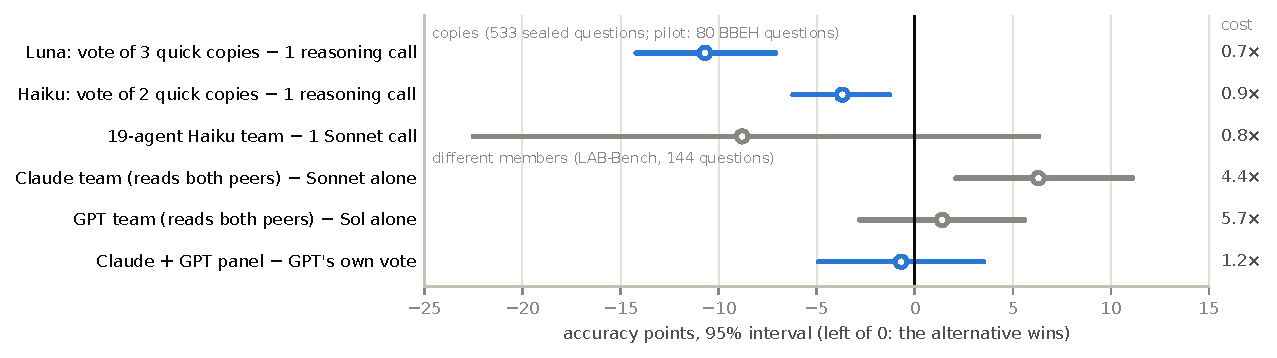
\includegraphics[width=\textwidth]{figs/fig_hero.pdf}
\caption{The collective minus its best alternative, in accuracy points with 95\% intervals; left of zero the alternative
wins, and the right column is the collective's cost as a multiple of the alternative's. Rows 1--2 (\status{confirmatory};
\nm{anchor.items.all} sealed questions): a vote of no-reasoning copies against one reasoning call of the same model at about
the same dollars. Row 3: the pilot's 19-agent Haiku team against one Sonnet call (\nm{pilot.items} BBEH questions). Rows
4--6 (LAB-Bench, \nm{lab.items} test questions): every member reading both teammates' answers against the team's best
single setting, and a preregistered Claude + GPT panel against GPT's own vote. Grey rows are descriptive.}
\label{fig:hero}
\end{figure*}

\section{Introduction}

Suppose an agent system has a fixed budget per task. It can ask a cheap model several times and vote, ask a
stronger or longer-reasoning model once, or ask several models and let a judge choose. Which should it buy first?
The answer depends on one quantity: how much the systems' failures are \emph{shared}. If every system fails the same
hard items, extra calls fail with them, and only a system that moves the hard items helps.

\paragraph{Six questions, in the order we met them.} (1) Can a team be compressed? A pruned 19-agent team was matched
by one stronger call (Section~\ref{sec:pilot}). (2) Why didn't 19 agents beat one call? Failures are dominated by shared
item difficulty, so width is capped by the items everyone fails (Sections~\ref{sec:pilot} and~\ref{sec:atlas}). (3) If
copies don't help, what does a dollar buy? Reasoning moves a system along the same difficulty axis, and the first effort
step of cheap models beat a dollar-matched vote in a preregistered test; verification selects among answers someone
produced and is capped by their coverage (Sections~\ref{sec:api} and~\ref{sec:verify}). (4) Do different members help
where copies don't? Only where the best member leaves room (Section~\ref{sec:members}). (5) Does a smarter coordination
rule help? Neither a learned rule for asking a teammate nor a recovery rule showed a gain we can credit to the rule; the
stronger member did (Section~\ref{sec:members}). (6) So the budget question reduces to choosing members
(Section~\ref{sec:alloc}).

\paragraph{Contributions.}
\begin{itemize}
\item \textbf{The Atlas}: one factor model fitted to \nm{atlas.swe.systems} SWE-bench Verified submissions,
\nm{atlas.ma.systems} MathArena configurations over \nm{atlas.ma.sets} competitions and \nm{atlas.lb.systems} LiveBench
models, with intervals for every systematic share and held-out tests of what it predicts about sets of systems:
coverage, the all-wrong tail and vote accuracy.
\item \textbf{Depth on public data}: \nm{p2.pairs} pairs of one model at two adjacent reasoning settings, pooled with
random effects, and a dollar-matched comparison of one deeper call against a wider vote (post hoc).
\item \textbf{Preregistered API studies}: a Phase~1 case where one reasoning call wins, and an anchor study on
\nm{anchor.items.all} sealed items with two confirmatory tests (AH2: the first effort step against the nearest-dollar
vote; AH3: the factor model's vote prediction), read once with frozen code.
\item \textbf{Team studies}: a 19-agent pilot; LAB-Bench teams for each provider with a preregistered rule for when to
ask a teammate and a preregistered cross-provider panel; and PHOENIX, a recovery rule for a lost member, on
\nm{phx.cases} cases of three science tables with every predictor sealed before scoring.
\item \textbf{A budget map}: the best team for each dollar and latency budget, chosen from stored calls at no cost.
\item \textbf{Process}: sealed items, single reads, preregistered stop rules and \nm{audits.count} independent audits,
for \nm{spend.total} of API spend in total. Every number in this paper is generated from a committed file and carries a
status (Appendix~\ref{app:repro}).
\end{itemize}

\section{Definitions}
\label{sec:defs}

We define each term in words first.
\textbf{Width}: more calls of the same setting, or of different systems, combined by a rule (a plurality vote) or a
selector. \textbf{Depth}: more reasoning per call (a higher effort or thinking budget) or a stronger tier.
\textbf{Verification}: choosing among candidate answers, by a judge model, a self-check, execution, or a label-free
rule such as Dawid--Skene~\cite{dawid1979}.

\paragraph{The factor model.} System $s$ answers item $i$ correctly with probability
$P_{si} = \sigma(a_s - \beta_s b_i)$, $\sigma(x) = 1/(1+e^{-x})$. The \emph{ability} $a_s$ is how good the system is
overall; the \emph{difficulty} $b_i$ is how hard the item is for everyone, the shared part of failure (scaled to mean 0
and standard deviation 1); the \emph{failure slope} $\beta_s$ is how sharply the system's success falls with
difficulty. Level L0 fixes $\beta_s = 1$. A \emph{family shock} $u_{f(s),i}$ adds a shared draw for systems of one
vendor; \emph{call luck} is what remains, identified only from repeated calls. Fits are penalised logistic
regressions (ridge \nm{design.ridge}), so items every system gets right or wrong keep finite difficulties.

\paragraph{Derived quantities.} The \emph{systematic share} $\mathrm{var}(b)/(\mathrm{var}(b)+\pi^2/3)$ is the share of
latent variation in success that items share ($\pi^2/3$ is the variance of the logistic call-level noise).
\emph{Coverage} of a set of systems is the share of items at least one member gets right: the ceiling of any rule that
returns one member's answer, as \citet{chen2026cofailure} also show; the \emph{all-wrong rate} is one minus coverage.
The \emph{vote ceiling} of one system is the share of items whose most common answer is right, the limit of infinitely
many repeats. \emph{Selection efficiency} $\eta = (\text{selected} - \text{best single})/(\text{coverage} - \text{best
single})$ is the share of the room above the best member that a selector reaches. A \emph{consensus inversion} is a
label-free rule rating a weaker system above the best one. \emph{Calibration by dilution}: adding near-random votes
shrinks a panel's calibration gap without improving its ranking (F13 in our findings ledger).

\paragraph{Statuses.} \status{confirmatory}: a preregistered test in a Holm family, read once on sealed items.
\status{preregistered-descriptive}: a preregistered quantity, read once, no pass/fail. \status{exploratory}: on sealed
items, not preregistered as a test. \status{post hoc}: chosen after the data were read, or on data not sealed for it;
all public-data analyses are post hoc in this sense, as are numbers computed after a read. Post hoc results are many and
uncorrected for multiplicity; we read them as descriptions, not tests.

\section{The pilot: nineteen agents and one call}
\label{sec:pilot}

Our first study pruned a team rather than measuring a lever (Figure~\ref{fig:hero}, row 3). Six Claude Haiku~5.5 proposers answered each question, six
critics read all six answers, six refiners revised, and one aggregator answered: 19 calls. On \nm{pilot.items} BBEH
questions the full team scored \nm{pilot.team.acc}\% at \nm{pilot.team.usd} per question; one Sonnet~5.5 call with
thinking off scored \nm{pilot.sonnet.acc}\% at \nm{pilot.sonnet.usd}, a difference of \nm{pilot.diff} points
(\nm{pilot.diff.lo} to \nm{pilot.diff.hi}; \status{exploratory}). The pruned teams tied within this noise.

The proposers' right-or-wrong records correlate at \nm{pilot.rho} on average, so six are worth \nm{pilot.neff}
independent answers (effective size $n/(1+(n-1)\rho)$, a measure of redundancy rather than a number of agents one could
deploy). A plurality vote of one proposer scores \nm{pilot.vote.k1}\% and of all six \nm{pilot.vote.k6}\% (averaged over
every set of proposers), while the chance that at least one is right rises from \nm{pilot.cover.k1}\% to
\nm{pilot.cover.k6}\%; independent errors at the same accuracy would give \nm{pilot.cover.indep}\%. Accuracy rose through
critique (\nm{pilot.stage.critique}\%) and refinement (\nm{pilot.stage.refine}\%) to \nm{pilot.stage.aggregate}\%: on the
\nm{pilot.rescue.low.n} questions where one or two proposers were right the team reached \nm{pilot.rescue.low.acc}\%, and
on the \nm{pilot.rescue.zero.n} where none was right it never recovered (\nm{pilot.rescue.zero.acc}\%). Checking selected
among answers someone produced; it did not create them. The stages were not ablated one by one. The next two sections ask
why failures are shared and what a dollar buys instead (Figure~\ref{fig:plateau}).

\begin{figure}[t]
\centering
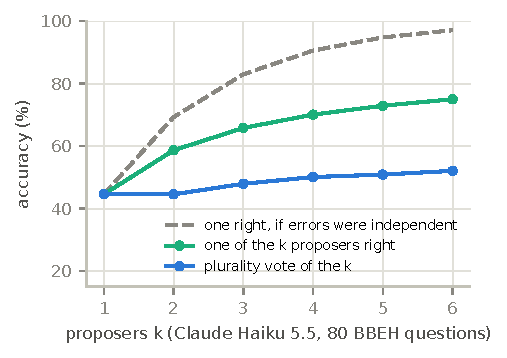
\includegraphics[width=\columnwidth]{figs/fig_plateau.pdf}
\caption{Six Claude Haiku~5.5 proposers in the pilot (\nm{pilot.items} BBEH questions): a plurality vote of $k$ proposers
(averaged over every set of $k$) against the share of questions at least one of the $k$ answered right, and that share
under independent errors at the same accuracy. Copies add coverage slowly and votes almost nothing.}
\label{fig:plateau}
\end{figure}

\section{The Atlas: what public data say about width and depth}
\label{sec:atlas}

\paragraph{Data.} SWE-bench Verified~\cite{jimenez2024swebench}: \nm{atlas.swe.systems} submissions on
\nm{atlas.swe.items} tasks, one run each, \nm{f17.systems} with per-task cost and step counts (mini-SWE-agent).
MathArena~\cite{balunovic2025matharena}: \nm{atlas.ma.systems} configurations on \nm{atlas.ma.items} final-answer
problems from \nm{atlas.ma.sets} competitions, usually four calls each, with answers grouped into classes by the
grader. LiveBench~\cite{white2024livebench}: \nm{atlas.lb.systems} models on \nm{atlas.lb.items} items of three binary
tasks, one call each, without answers or costs. Each benchmark is fitted on its own. All Atlas numbers are
\status{post hoc}.

\subsection{Failures are mostly shared}

The systematic share is \nm{p6.swe.est} on SWE-bench Verified (item bootstrap \nm{p6.swe.ilo}--\nm{p6.swe.ihi}; over
\nm{design.halves} random halves of the systems, \nm{p6.swe.hmin}--\nm{p6.swe.hmax}), \nm{p6.ma.est} on MathArena
(\nm{p6.ma.ilo}--\nm{p6.ma.ihi}) and \nm{p6.lb.est} on LiveBench (\nm{p6.lb.ilo}--\nm{p6.lb.ihi}); our Phase~1 BBEH panel
of four arms sits lower at \nm{p6.bbeh.est} (\nm{p6.bbeh.ilo}--\nm{p6.bbeh.ihi}; Figure~\ref{fig:share}). On the
\nm{f17.systems} SWE-bench submissions with per-task data, difficulty alone implies \nm{f17.difficulty.share}\% of the
mean pairwise failure correlation (\nm{f17.corr.l0} of \nm{f17.corr.obs}); two systems of one company add only
\nm{f17.samecompany} of residual correlation. All \nm{f17.systems} fail \nm{f17.allwrong.obs}\% of tasks, against
\nm{f17.allwrong.indep}\% if they failed independently.

\begin{figure}[t]
\centering
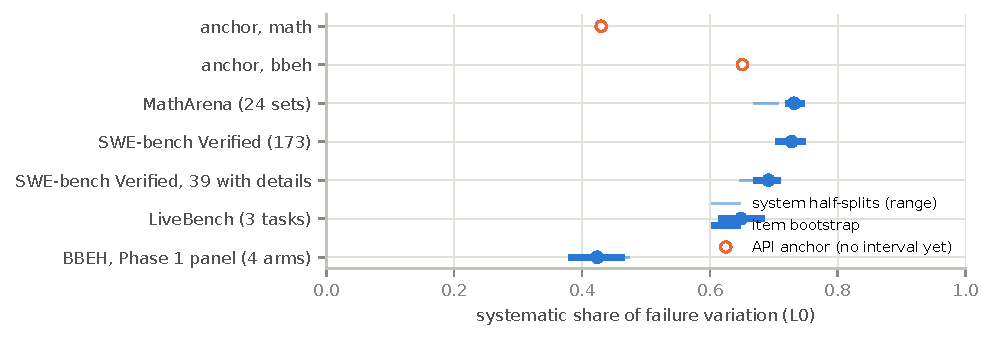
\includegraphics[width=\columnwidth]{figs/fig_share.pdf}
\caption{Systematic failure share per source (L0): item-bootstrap 95\% interval (thick) and the range over system
half-splits (thin; each half fitted on its own). The anchor's shares (hollow) await the gold files for an interval.}
\label{fig:share}
\end{figure}

\subsection{Width is capped by the shared tail}

\paragraph{Coverage and the all-wrong tail.} Fitting difficulties on half the systems and each held-out system's ability
on half the tasks, the model predicts the coverage of held-out \nm{design.sets.lo}--\nm{design.sets.hi} system sets on held-out SWE-bench tasks within
\nm{a5.swe.model.lo}--\nm{a5.swe.model.hi} points; independence misses by \nm{a5.swe.indep.lo}--\nm{a5.swe.indep.hi}.
\citet{chen2026cofailure} report that a calibrated one-factor copula underprices the all-wrong tail by about
\nm{cited.cofailure.under}$\times$
on open-ended mathematics. We give the factor model and the copula the same information, the calibration tasks only: the
factor model draws an unknown test task's difficulty from the calibration tasks' difficulties, the copula fits its
correlation to the calibration tasks' pairwise failures. For all \nm{p8.swe.members} held-out SWE-bench systems on
\nm{p8.swe.items} held-out tasks the observed all-wrong rate is \nm{p8.swe.obs}\% (Clopper--Pearson
\nm{p8.swe.cplo}--\nm{p8.swe.cphi}); the factor model predicts \nm{p8.swe.model}\% (observed over predicted
\nm{p8.swe.rmodel}, \nm{p8.swe.rmodello}--\nm{p8.swe.rmodelhi}), the copula \nm{p8.swe.copula}\%
(\nm{p8.swe.rcopula}$\times$) and independence \nm{p8.swe.indep}\% (Figure~\ref{fig:tail}). The factor model's free
distribution of difficulties carries the tail that a Gaussian latent factor misses. On the small MathArena sets
(\nm{design.p8.ma.items.lo}--\nm{design.p8.ma.items.hi} test problems) both models underpredict the 5-system tail, on
\nm{p8.ma.model.under} and \nm{p8.ma.copula.under} of \nm{p8.ma.sets} sets; the math tail is unresolved.

\paragraph{Votes of one system.} A vote of two calls cannot gain in expectation (a right--wrong split is a tie), so gains
start at three. The factor model's \emph{vote rule} predicts a $k$-vote from one-call success $p$, the share $z$ of
failures that abstain (abstentions are non-votes) and the chance $q$ that two wrong answers coincide. Cross-fitted on
\nm{p1.all.cells} (system, set) cells with three calls in \nm{p1.all.sets} sets, its mean absolute vote-gain error is
\nm{p1.all.rule} points against \nm{p1.all.zero} for the zero-gain predictor ``votes add nothing''; predicted and
observed gains correlate at \nm{p1.all.corr}, and the gain's squared error is smaller by \nm{p1.all.msed} points$^2$
(\nm{p1.all.msedlo} to \nm{p1.all.msedhi}; item noise adds the same variance to both and cancels). But the rule
overstates gains (\nm{p1.pred.predgain} predicted, \nm{p1.pred.obsgain} observed where it predicts \nm{design.gainpoints}
or more), and on the 3-vote accuracy itself it is worse than zero-gain (mean absolute error \nm{p1.all.levrule} against
\nm{p1.all.levzero} points; squared error larger by \nm{p1.all.levmsed} points$^2$, \nm{p1.all.levmsedlo} to
\nm{p1.all.levmsedhi}). The rule ranks where votes pay; it does not yet price them.

\paragraph{Votes across systems.} Votes pay most when weak systems with different strengths are mixed. On
\nm{p7.k3.panels} panels of three and \nm{p7.k5.panels} of five MathArena systems with one-call accuracy
\nm{design.weak.lo}--\nm{design.weak.hi}, the plurality of one call each gains \nm{p7.k3.gain} and \nm{p7.k5.gain} points
over a random member. Cross-fitted, the factor model predicts the panel vote with bias \nm{p7.k3.bias} and
\nm{p7.k5.bias} points and absolute error \nm{p7.k3.model} and \nm{p7.k5.model}, against \nm{p7.k3.zero} and
\nm{p7.k5.zero} for zero-gain and \nm{p7.k3.indep} and \nm{p7.k5.indep} for independence; it is closer than zero-gain in
\nm{p7.k3.setszero} and \nm{p7.k5.setszero} of \nm{p7.k3.sets} sets, and closer than independence in
\nm{p7.k3.setsindep} and \nm{p7.k5.setsindep}. Where composition matters, the model prices it without bias;
independence overstates it and zero-gain ignores it.

\subsection{Depth moves ability, not the failure pattern}

For each of \nm{p2.pairs} public pairs of one model at two adjacent reasoning settings (\nm{p2.models} models, some on two
benchmarks; difficulties from every other system), we fit both settings' ability and slope on the items both answered
(Figure~\ref{fig:depth}). Pooled with random effects, ability rises by \nm{p2.all.da.pooled} logits
(\nm{p2.all.da.lo}--\nm{p2.all.da.hi}; between-pair variance \nm{p2.all.da.tau}); the slope changes by
\nm{p2.all.db.pooled} (\nm{p2.all.db.lo}--\nm{p2.all.db.hi}; between-pair variance \nm{p2.all.db.tau}). One pair per
model and benchmark (\nm{p2.modelbench} pairs) gives \nm{p2.one.da.pooled} and \nm{p2.one.db.pooled}. Held out, the
higher setting's calls are predicted better by the lower setting plus one shift than by a refit that may also change
the slope (log loss per call \nm{p2.all.slope.pooled} in favour of the shift, \nm{p2.all.slope.lo}--\nm{p2.all.slope.hi})
and far better than by its base rate (\nm{p2.all.base.pooled} nats per call). The difficulties are the population's, so
this says the higher setting fails the items that are hard for everyone; the lower setting's own item outcomes plus a
shift predict no better (\nm{p2.all.own.pooled}, \nm{p2.all.own.lo} to \nm{p2.all.own.hi}). Two pairs left out after a
look at output tokens (one setting of unknown order, one different checkpoint) are shown in the extension report and
were never pooled.

\paragraph{Depth against width at equal dollars (post hoc).} For \nm{p3.all.k} MathArena pairs whose lower setting has
three or more calls, one call at the higher setting minus the vote of the lower setting with the nearest dollars per
item (the 3-vote in every pair) is \nm{p3.all.pooled} points (\nm{p3.all.lo}--\nm{p3.all.hi}); on the \nm{p3.near.k}
pairs priced within a factor of \nm{design.near} it is \nm{p3.near.pooled} (\nm{p3.near.lo}--\nm{p3.near.hi}; Figure~\ref{fig:dw}).
The step pays where a model starts low and about nothing at the top of its range: \nm{p3.geminimed.diff} points for
Gemini~3.1~Pro medium to default and \nm{p3.opus.diff} for Opus~5.5 high to max. We logged, before it is read, that this
predicts about zero for the preregistered CD2 test of a top Haiku effort step. Price matters as much: on SWE-bench Verified
MiniMax~M2.5 (high) resolves \nm{f18.minimax.acc}\% at \nm{f18.minimax.usd} per task against \nm{f18.opus.acc}\% at
\nm{f18.opus.usd} for Claude Opus~4.5 (high), \nm{f18.price.ratio}$\times$ the price for one point
(Figure~\ref{fig:tail}, right).

\begin{figure}[t]
\centering
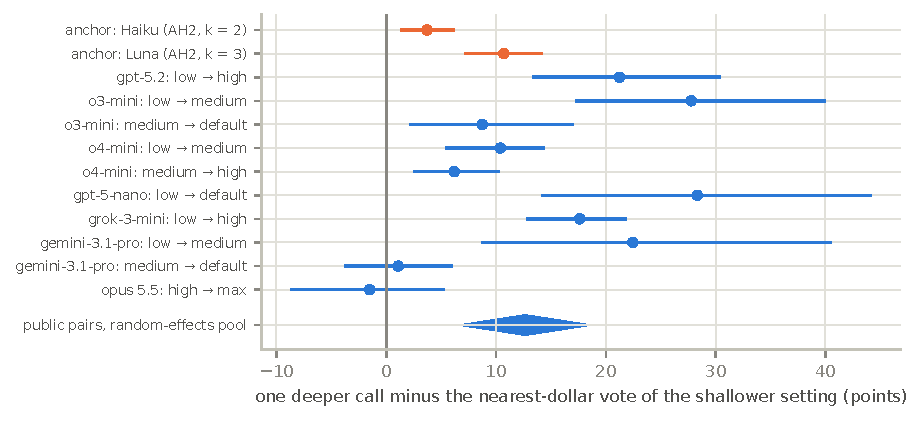
\includegraphics[width=\columnwidth]{figs/fig_dw.pdf}
\caption{One deeper call minus the nearest-dollar vote of the shallower setting: the anchor's confirmatory AH2 (orange,
fresh sealed items, the first effort step of two cheap models) and public MathArena pairs (blue, post hoc) with
item-bootstrap 95\% intervals and their random-effects pool.}
\label{fig:dw}
\end{figure}

\section{Preregistered API studies}
\label{sec:api}

\paragraph{Phase 1: the saturated case.} On \nm{phase1.items} sealed BBEH items~\cite{kazemi2025bbeh}, one GPT-6.1 Sol
call at low reasoning was right \nm{f3.sol.acc}\% of the time at \nm{f3.sol.usd} per call; Claude Sonnet~5.5 without
reasoning \nm{f3.sonnet.acc}\% at \nm{f3.sonnet.usd} (\status{preregistered-descriptive}). Width bought little: \nm{f1.calls}
Haiku calls are worth \nm{f1.neff5} independent calls (repeat correlation \nm{f1.rho}), their plurality reached
\nm{f4.haiku5}\%, a \nm{f4.panel.calls}-call mixed panel \nm{f4.panel12}\%, and none of \nm{f4.cascades} cascade settings came within
\nm{f4.within} points of Sol at \nm{f4.dollars}$\times$ its dollars (\status{exploratory}/\status{post hoc}). The
confirmatory cascade test (H7) passed non-inferiority to Sonnet (\nm{f5.diff} points) only by escalating
\nm{f5.escalates}\% of items. Sol's accuracy is not answer memory: \nm{f7.perturbed} of \nm{f7.of} perturbed items right.
The Sol--Sonnet gap mixed vendor and reasoning, which motivated the anchor.

\paragraph{The anchor.} \nm{anchor.items.bbeh} BBEH items (linguistic puzzles, cartoon captions, word sorting, causal
judgement) and \nm{anchor.items.math} arXivMath problems were sealed before any call. Arms: Claude Haiku~5.5 (off, low,
high), Sonnet~5.5 (off, low), GPT-6 Luna (none, low, medium), GPT-6.1 Sol (low, medium), most with three calls per
item; dollars are measured at list prices. Each block was read once with frozen code; Holm at 5\% over the two tests
that kept power of at least \nm{design.power.min} (AH2, AH3).

\emph{AH2 (\status{confirmatory}, passes; $p = \nm{ah2.p.holm}$).} Raising a cheap model's reasoning one step beat
repeating its no-reasoning call at the nearest measured dollars: Haiku at effort low against the Haiku-off
\nm{ah2.haiku.k}-vote by \nm{ah2.haiku.diff} points (\nm{ah2.haiku.lo}--\nm{ah2.haiku.hi}), Luna at reasoning low against
the Luna-none \nm{ah2.luna.k}-vote by \nm{ah2.luna.diff} (\nm{ah2.luna.lo}--\nm{ah2.luna.hi}); the deeper call cost
\nm{ah2.haiku.ratio}$\times$ and \nm{ah2.luna.ratio}$\times$ as much. For Haiku the 2-vote equals one call in
expectation, so this shows that effort low beats effort off at slightly more dollars, not that depth beats a wider vote;
against the dearer 3-vote the difference is \nm{ah2.haiku.vs3} (\nm{ah2.haiku.vs3lo}--\nm{ah2.haiku.vs3hi}), not tested.
The effect sits mainly in word sorting (and linguistic puzzles for Luna; computed after the read). The decision as frozen:
for cheap models on these items, buy the first effort step before width. It covers neither higher steps nor other tasks.

\emph{AH3, the vote rule (\status{confirmatory}, passes).} Cross-fitted on single calls, the factor model predicted the
six 3-call arms' 3-vote accuracy with mean absolute error \nm{ah3.mae} points (upper bound \nm{ah3.upper}) and their gain
over one call within \nm{ah3.gain} (upper bound \nm{ah3.gainupper}). The gains were small (\nm{ah3.gain.lo} to
\nm{ah3.gain.hi} points) and zero-gain also meets the limits (gain error \nm{p1.anchor.zero} against \nm{p1.anchor.rule}),
so AH3 shows accuracy where votes gain little; P1 above finds the same rule overstating larger gains.

\emph{AH1 and AH4 (\status{exploratory}).} Sonnet's effort-low setting closed none of the
\nm{ah1.gap}-point gap to Sol low ($R = \nm{ah1.r}$, \nm{ah1.lo} to \nm{ah1.hi}), so the vendor--reasoning confound stays
open. The Sol judge's selection efficiency was \nm{ah4.easy} on easy items and \nm{ah4.hard} on hard ones (difference
\nm{ah4.diff}, \nm{ah4.lo}--\nm{ah4.hi}), the predicted direction, with a ratio whose hard-half denominator is small.

\paragraph{The depth study.} A preregistered study of Haiku at every reasoning effort (research/v4/cd/read.md)
finds that accuracy gains flatten by the second-highest effort; the drop at the highest effort is within its interval
and coincides with calls cut at the output limit.

\section{Verification}
\label{sec:verify}

\paragraph{Label-free selection.} With repeats, Dawid--Skene rated Sol at \nm{f11.sol.est}\% on Phase~1 against a true
\nm{f11.sol.true}\% (\status{exploratory}); on the anchor its pooled variant put Sonnet at \nm{lf.sonnet.est}\% against
a true \nm{lf.sonnet.true}\%, and its answers (\nm{lf.answer}\%) stayed below one Sol low call (\nm{anchor.sol.all}\%).
A simulation map (Figure~\ref{fig:labelfree}) shows when this happens: with one strong system among weak ones and one
call each, plain Dawid--Skene ranks a weak system first in \nm{p4.sim.lone.ds.inv}\% of panels; a fixed label space
removes the inversion in the simulation (\nm{p4.sim.lone.fixed.inv}\%) but still loses \nm{p4.sim.lone.fixed.loss}
points to the strong system. On MathArena the fixed label space does not help: beside a lone strong system it ranks
another system first in \nm{p4.ma.lone.fixedinv.lo}--\nm{p4.ma.lone.fixedinv.hi}\% of panels, against
\nm{p4.ma.lone.inv.lo}--\nm{p4.ma.lone.inv.hi}\% for plain Dawid--Skene. At matched calls (three systems with one call
each, against the best system's own 3-vote, the best chosen with labels) every policy loses beside a lone strong system
(plurality \nm{p4.ma.match.lone.plur} points, plain Dawid--Skene \nm{p4.ma.match.lone.ds}) and none gains among
competent ones (plurality \nm{p4.ma.match.comp.plur}, plain Dawid--Skene \nm{p4.ma.match.comp.ds}, fixed labels
\nm{p4.ma.match.comp.fixed}).

\paragraph{The anchor's judge, and why it cannot test judges.} On the anchor's BBEH items the Sol low judge, choosing
among the answers of two cheap pools, reached \nm{judge.sol.bbeh.acc}\%: \nm{judge.sol.bbeh.vsbest} points above the best
pool arm (\nm{judge.sol.bbeh.vsbestlo}--\nm{judge.sol.bbeh.vsbesthi}), selection efficiency \nm{judge.sol.bbeh.eta}
(\nm{judge.sol.bbeh.etalo}--\nm{judge.sol.bbeh.etahi}). Sol low answering alone scored \nm{anchor.sol.bbeh}\%, so the
judge sat \nm{judge.sol.below} points below it (\nm{judge.sol.vsown.lo} to \nm{judge.sol.vsown.hi}) at
\nm{judge.sol.vsown.ratio}$\times$ the dollars (Figure~\ref{fig:judge}; \status{post hoc}, computed after the read).
But the pools covered only \nm{judge.sol.bbeh.coverage}\% of the items: even a perfect selector over them would have lost
to Sol alone. The comparison measures the pools, not the judge's signal; a test of judges needs pools whose coverage
exceeds the judge model's own accuracy. On math the judge was capped by \nm{judge.sol.math.coverage}\% coverage.

\begin{figure}[t]
\centering
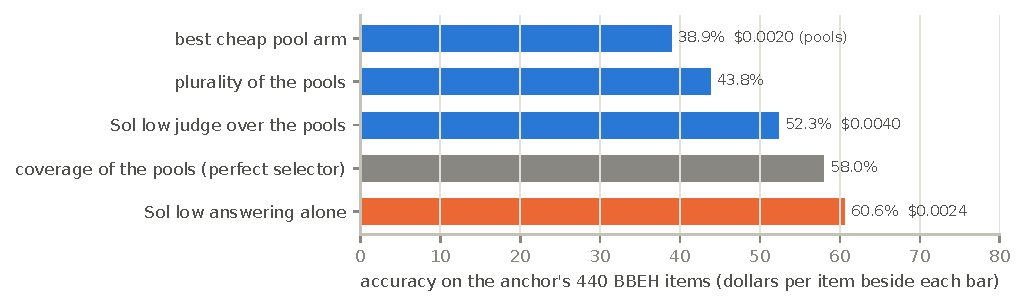
\includegraphics[width=\columnwidth]{figs/fig_judge.pdf}
\caption{The anchor's BBEH verification read: a judge over cheap pools against the judge model answering alone. The
pools' coverage (grey) is below the judge model's own accuracy, which caps every selector over them.}
\label{fig:judge}
\end{figure}

\paragraph{The price of verification on public data.} A perfect selector over random \nm{design.sets.lo}--\nm{design.sets.hi} system SWE-bench sets adds
\nm{p5.swe.room2}--\nm{p5.swe.room5} points over the best member, at \nm{p5.swe.price2}--\nm{p5.swe.price5} of extra
spend per point per task. With the anchor's best measured efficiency, a judge over such a set beats the most accurate
single submission at no more of its dollars in at most \nm{p5.swe.beat.sol}\% of sets (a perfect selector in at most
\nm{p5.swe.beat.perfect}\%, judge calls unpriced). On MathArena the room is \nm{p5.ma.room.lo}--\nm{p5.ma.room.hi}
points because the top systems are close to perfect.

\paragraph{Self-checks and execution.} Sol accepted \nm{check.sol.accept}\% of its own anchor answers (AUROC
\nm{check.sol.auroc}); Haiku \nm{check.haiku.accept}\% (AUROC \nm{check.haiku.auroc}). On SWE-bench the step count of a
run ranks its own successes with median AUROC \nm{f18.stepauroc}; a cascade that escalates on step count never
escalates once its threshold is fitted. Execution-based checks on code are part of the open-weight testbed.

\begin{figure}[t]
\centering
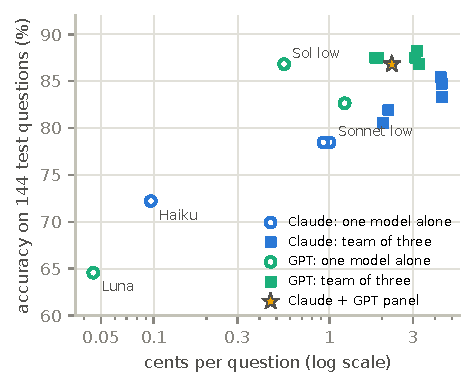
\includegraphics[width=\columnwidth]{figs/fig_lab.pdf}
\caption{LAB-Bench test (\nm{lab.items} questions): accuracy against cost per question. Open circles: one model alone;
squares: each provider's five team methods (a vote, everyone thinking again, asking the best peer, reading both peers, the
learned rule); star: the preregistered Claude + GPT panel. One GPT-6.1 Sol call at low effort matches every team.}
\label{fig:lab}
\end{figure}

\begin{figure}[t]
\centering
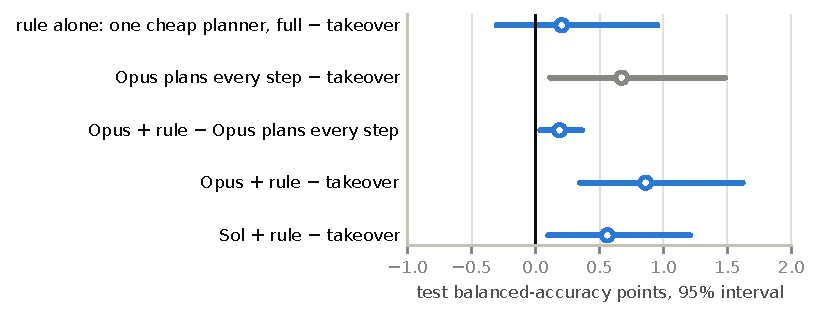
\includegraphics[width=\columnwidth]{figs/fig_phx.pdf}
\caption{PHOENIX on \nm{phx.cases} cases of three science tables: sealed test balanced-accuracy points, paired by case
(each arm case is the mean of two draws). Blue rows are preregistered contrasts; the grey row is post hoc. The rule alone is
not resolved, and most of the gain over takeover comes from the stronger planner.}
\label{fig:phx}
\end{figure}

\section{Different members and coordination rules}
\label{sec:members}

\paragraph{Different members.} If copies fail together, members that fail differently should help (Figure~\ref{fig:lab}). On \nm{lab.items}
held-out LAB-Bench questions (DNA-sequence manipulation and protocol troubleshooting), each provider fielded one cheap model
and one strong model at two reasoning efforts: Claude Haiku~5.5 with Sonnet~5.5 at low and medium effort (two models,
three settings), and GPT-6 Luna with GPT-6.1 Sol at low and medium. With every member reading both teammates' answers
before revising, the Claude team scored \nm{lab.claude.review.acc}\% against \nm{lab.claude.single.acc}\% for Sonnet low
alone, \nm{lab.claude.reviewminus} points (\nm{lab.claude.reviewminus.lo} to \nm{lab.claude.reviewminus.hi};
\status{post hoc}) at \nm{lab.claude.review.ratio}$\times$ the cost; a plain vote of the three first answers gained
\nm{lab.claude.voteminus} (\nm{lab.claude.voteminus.lo} to \nm{lab.claude.voteminus.hi}). Sol low alone scored
\nm{lab.gpt.single.acc}\% at \nm{lab.gpt.single.usd} per question, and no GPT team beat it by a resolved margin (every
member reading both teammates: \nm{lab.gpt.reviewminus}, \nm{lab.gpt.reviewminus.lo} to \nm{lab.gpt.reviewminus.hi}). The
best Claude team (\nm{lab.claude.peer.acc}\% at \nm{lab.claude.peer.usd}) stayed below that one Sol call. A preregistered
panel mixing the providers, chosen on practice questions and replayed from stored calls at no cost, scored
\nm{lab.mix.acc}\% at \nm{lab.mix.usd}: \nm{lab.mix.gpt} points against GPT's own vote (\nm{lab.mix.gpt.lo} to
\nm{lab.mix.gpt.hi}) and \nm{lab.mix.claude} against Claude's (\nm{lab.mix.claude.lo} to \nm{lab.mix.claude.hi}). The claim
needed both to be positive and is not supported (\status{confirmatory}). The two providers refused disjoint questions, too
few to matter for a vote.

\paragraph{A learned rule for when to ask a teammate.} After its first answer each member could stop, think again alone,
or ask one teammate. A per-member rule was fitted on practice questions, frozen, and read once; it had to be cheaper than
every member thinking again, with the lower 95\% bound of its accuracy difference above $-3$ points. Neither team's rule
passed: Claude \nm{lab.claude.primary} (\nm{lab.claude.primary.lo} to \nm{lab.claude.primary.hi}) at
\nm{lab.claude.policy.usd} against \nm{lab.claude.reflect.usd} per question, and GPT \nm{lab.gpt.primary}
(\nm{lab.gpt.primary.lo} to \nm{lab.gpt.primary.hi}) (\status{confirmatory}). Claude's rule did worse than random choices
of the same number of calls (\nm{lab.claude.random}, \nm{lab.claude.random.lo} to \nm{lab.claude.random.hi}), and GPT's
mostly reproduced the plain vote.

\paragraph{Recovering a lost member (PHOENIX; Figure~\ref{fig:phx}).} Three agents build a classifier on a public science table (forest cover
type, MiniBooNE neutrino events or HIGGS collisions), and halfway through one member is shut down and its model withdrawn.
Three recoveries ran under the same caps on dollars, calls, tools and CPU time: ordinary takeover by the next model, a
planner model choosing every step, and PHOENIX, which ranks candidate plans by expected gain per dollar along the
workflow's dependencies. Every recovered predictor was sealed and then scored once on a held-out split
(\nm{phx.recoveries} recoveries, balanced-accuracy points). Where the rule can be isolated, with one cheap model doing
everything, PHOENIX minus takeover is \nm{phx.main} (\nm{phx.main.lo} to \nm{phx.main.hi}; \status{confirmatory}, not
resolved). With Claude Opus~5.5 planning it beats takeover by \nm{phx.claude} (\nm{phx.claude.lo} to \nm{phx.claude.hi}),
but Opus choosing every step without the rule already gains \nm{phx.planner} (\nm{phx.planner.lo} to \nm{phx.planner.hi};
\status{post hoc}); the rule adds \nm{phx.rule} (\nm{phx.rule.lo} to \nm{phx.rule.hi}) at \nm{phx.usd.full} against
\nm{phx.usd.llm} per recovery. With GPT-6.1 Sol planning the gain over takeover is \nm{phx.gpt} (\nm{phx.gpt.lo} to
\nm{phx.gpt.hi}) and fragile, and two draws of the same method on one case differed by up to \nm{phx.drawnoise} points.
The planner model mattered; the rule's own value is not shown.

\begin{figure*}[t]
\centering
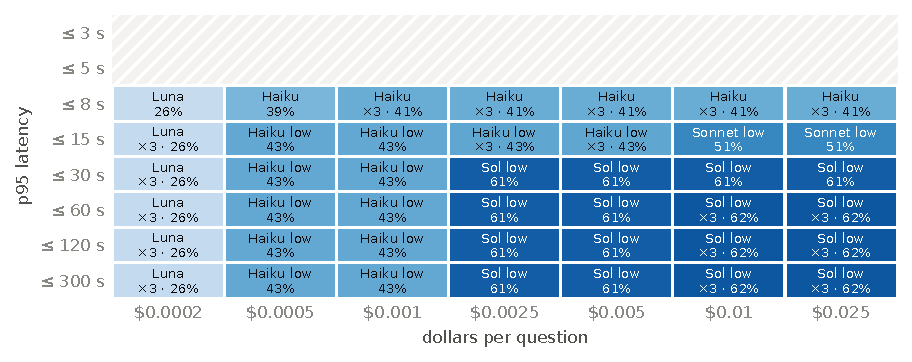
\includegraphics[width=\textwidth]{figs/fig_map.pdf}
\caption{The budget map on the anchor's BBEH questions: the most accurate team within each dollar budget (columns) and
95th-percentile latency budget (rows), chosen by replaying stored calls. Shading is its accuracy; ``$\times$3'' marks a vote of
three calls of one model; hatched rows have no team fast enough. Every winner is a single model.}
\label{fig:map}
\end{figure*}

\section{Choosing members per budget}
\label{sec:alloc}

Because every call is stored, every team in this paper is rescored by replay at no cost, and the best team for each dollar
and latency budget can be chosen from calls already made (Figure~\ref{fig:map}). On the anchor's BBEH questions \nm{map.cells} budget cells have a
feasible team, and in every one the winner is a single model: one call in \nm{map.single} cells and a vote of its own
copies in \nm{map.vote}. Chosen on half the questions and scored on the other half, the choice loses
\nm{map.regret.lo}--\nm{map.regret.hi} points on average against the best team for the held-out half
(\status{exploratory}). This is stability within one benchmark, not transfer to a new task.

\section{The open-weight testbed (design; results pending)}
\label{sec:testbed}

The testbed varies precision (BF16, W8, W4, W3), size (Qwen3.5 2B, 4B, 9B) and thinking budget (off, 1k, 4k) with
several samples per item on \nm{testbed.items.all} items (\nm{testbed.items.bbeh} BBEH, \nm{testbed.items.math}
competition math, \nm{testbed.items.code} LiveCodeBench), so width, depth and verification can be bought at measured GPU
cost. Its preregistration (T1--T5) has power by simulation of \nm{testbed.power.t1} (T1: the W4 loss survives voting on
hard items), \nm{testbed.power.t2} (T2), \nm{testbed.power.t3} (T3: depth against cost-matched width),
\nm{testbed.power.t4} (T4: judge coupling to difficulty) and \nm{testbed.power.t5} (T5, exploratory: compositional
prediction) (\status{design}). The pilot is estimated at \nm{testbed.gpu.pilot} of GPU time. No GPU has run yet; no
result is reported.

\section{Related work}
\label{sec:related}

\paragraph{Shared failure and its ceiling.} \citet{chen2026cofailure} show that any routing, voting or cascade policy
returning one model's answer is bounded by one minus the share of queries every model fails, certify that share from a
graded set, and find that a one-factor copula underprices it on open-ended mathematics; they exclude thinking variants
and do not hold dollars fixed. We take the ceiling as given and ask how depth moves it and at what price.
\citet{kim2025correlated} measure correlated errors across hundreds of models without an item-difficulty term;
\citet{turkmen2026ensemble} prove an error floor under a Gaussian latent factor; \citet{denisovblanch2026consensus}
find that polling does not improve truthfulness because errors are shared. \citet{ge2026psychometrics} fit an
ability-minus-difficulty model to agentic coding leaderboards to predict tasks and agents; we use the same scale for
composition.

\paragraph{Width.} \citet{chen2024morecalls} show that vote accuracy can rise and then fall with more calls of one model
on a mix of easy and hard queries; they count calls, not dollars. \citet{chen2025llmselector} assign different models to
the modules of a compound system with a labelled search, which can beat any single model; this is role allocation, not
parallel width.

\paragraph{Verification and cascades.} \citet{singhi2025solve} find self-consistency more compute-efficient than
generative verification at most practical budgets, with verification ahead only at many times the compute; our
comparator is the judge model's own answer at measured dollars. Conformal cascades~\cite{dou2026conformal} need
labelled calibration data; C3PO~\cite{valkanas2025c3po} anchors a label-free cascade on the strongest model's answers
and so inherits its errors. Learn-then-Test~\cite{angelopoulos2021ltt} gives the risk control we plan for a runtime
router.

\section{Limitations}
\label{sec:limits}

Models and prices are those of October 2026, and public leaderboards mix scaffolds and dates. Most Atlas results are
post hoc and uncorrected for the many comparisons made. Contamination cannot be ruled out: BBEH has been public since
2025, so ``fresh'' means new to this project, and LiveCodeBench predates the testbed's models. The API studies are small
(\nm{anchor.items.all} items in the anchor) and use two vendors; the AH2 decision covers the first effort step for cheap
models on these items only; beyond it the depth study describes flattening gains but does not test depth against
width. The anchor's judge test was capped by its pools. The team studies are small (\nm{lab.items} LAB-Bench test
questions, \nm{phx.cases} PHOENIX cases on tables near their accuracy ceiling), several team comparisons are post hoc, and
the budget map's stability is measured within one benchmark. Answer
format moves the difficulty axis~\cite{chen2026cofailure}; our anchor tasks are free-form. The all-wrong tail on small
math sets is not resolved. The anchor's systematic shares have no interval until the gold files are restored.

\section{Conclusion and next steps}
\label{sec:conclusion}

Which members a system calls matters more than how it organizes them. On the data we have, failures are mostly shared, and a factor model with one free difficulty per item prices the shared
tail on code better than a one-factor copula given the same data. Reasoning moves a system along the shared difficulty
axis without changing which items it fails. The first reasoning step of cheap models beat a dollar-matched vote of their
no-reasoning calls on sealed items; whether depth beats width beyond that step is open, and our public pairs predict
about zero at the top of a model's range. Selection by agreement did not beat the best system's own vote at matched
calls, and a test of judges still needs pools that cover more than the judge answers alone. Different members helped
only where the best member left room, and smarter coordination rules, for asking a teammate or for recovering a lost
member, showed no gain we can credit to the rule. A preregistered handoff test, how much of a strong model's
accuracy a cheaper team completes from the strong model's partial reasoning, has run and is not yet read. The next steps (roadmap in
research/v4/roadmap.md): \nm{plan.items}+ items across \nm{plan.families} or more task families including agentic ones,
with a time-split replication; a third vendor used once on the frozen design; the open-weight testbed; batch and cache
pricing; and a budget allocator that turns a \nm{plan.pilot.lo}--\nm{plan.pilot.hi} item pilot and a price table into a
depth, width and verification mix with predicted accuracy, cost and uncertainty.

\bibliographystyle{icml2026}
\bibliography{refs}

\appendix

\section{Reproducibility}
\label{app:repro}

\paragraph{Preregistration.} Every paid run carried a committed \texttt{prereg:} block (question, prediction, kill rule,
decision) that code checked before the run could spend; the full texts are in the repository's research/ folder.
Tests whose simulated power at the chosen $n$ fell below \nm{design.power.min} were reported as exploratory.

\paragraph{Audits.} An independent audit read every design and every paid run's outcome before the next step:
\nm{audits.count} audits, with \nm{audits.go} GO, \nm{audits.adjust} ADJUST and \nm{audits.stop} STOP verdicts; every
ADJUST was resolved before further spend.

\paragraph{Cost.} Total API spend \nm{spend.total} over \nm{runs.count} runs, under hard per-account caps enforced in
code. Every call is stored, so every team in this paper is rescored by replay at no cost. The per-run ledger and the
status of every number in the paper are generated in the repository (paper/runs\_table.tex, paper/numbers\_table.tex).

\section{Additional figures}
\label{app:figs}

\begin{figure*}[t]
\centering
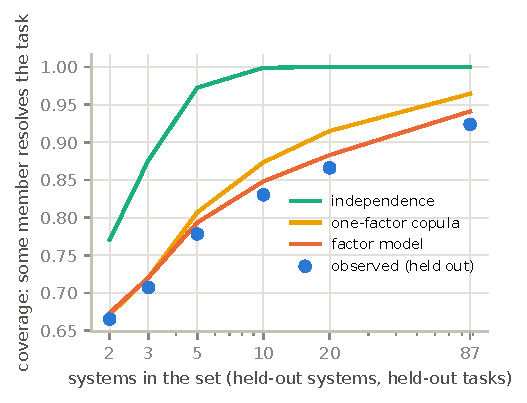
\includegraphics[width=0.62\textwidth]{figs/fig_tail.pdf}\hfill
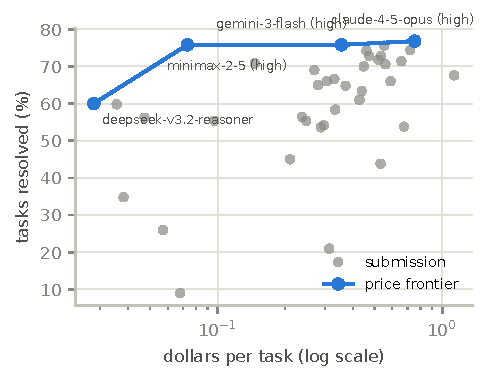
\includegraphics[width=0.36\textwidth]{figs/fig_frontier.pdf}
\caption{Left: coverage of sets of held-out SWE-bench Verified systems on held-out tasks, observed and predicted from the
calibration tasks only (P8). Right: tasks resolved against dollars per task, SWE-bench Verified submissions with costs;
the price frontier in blue (A7).}
\label{fig:tail}
\end{figure*}

\begin{figure*}[t]
\centering
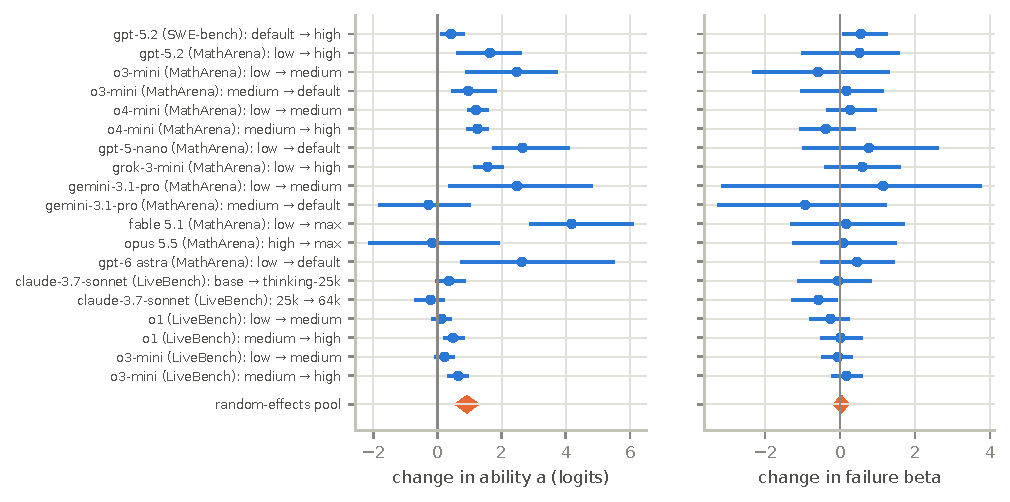
\includegraphics[width=\textwidth]{figs/fig_depth.pdf}
\caption{One model at two adjacent reasoning settings (P2): change in ability $a$ and in failure slope $\beta$ with
item-bootstrap 95\% intervals, and the DerSimonian--Laird random-effects pool (diamond).}
\label{fig:depth}
\end{figure*}

\begin{figure*}[t]
\centering
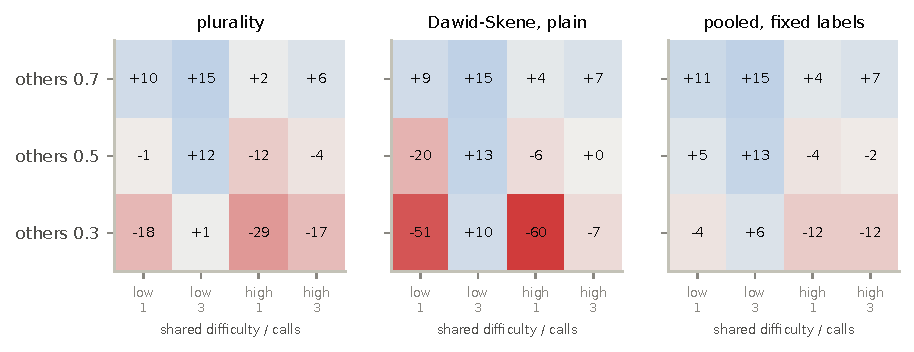
\includegraphics[width=\textwidth]{figs/fig_labelfree.pdf}
\caption{Label-free selection, simulation map (P4): gain over the best system (points) when one system at
\nm{design.p4.top} sits among others at \nm{design.p4.others0}, \nm{design.p4.others1} or \nm{design.p4.others2}, at low
or high shared difficulty (systematic share \nm{design.p4.share0} or \nm{design.p4.share1}), with one or three calls per
system; averaged over \nm{design.p4.systems0}, \nm{design.p4.systems1} and \nm{design.p4.systems2} systems.}
\label{fig:labelfree}
\end{figure*}

\end{document}
